\documentclass[11pt]{article}

    \usepackage[breakable]{tcolorbox}
    \usepackage{parskip} % Stop auto-indenting (to mimic markdown behaviour)
    
    \usepackage{iftex}
    \ifPDFTeX
    	\usepackage[T1]{fontenc}
    	\usepackage{mathpazo}
    \else
    	\usepackage{fontspec}
    \fi

    % Basic figure setup, for now with no caption control since it's done
    % automatically by Pandoc (which extracts ![](path) syntax from Markdown).
    \usepackage{graphicx}
    % Maintain compatibility with old templates. Remove in nbconvert 6.0
    \let\Oldincludegraphics\includegraphics
    % Ensure that by default, figures have no caption (until we provide a
    % proper Figure object with a Caption API and a way to capture that
    % in the conversion process - todo).
    \usepackage{caption}
    \DeclareCaptionFormat{nocaption}{}
    \captionsetup{format=nocaption,aboveskip=0pt,belowskip=0pt}

    \usepackage{float}
    \floatplacement{figure}{H} % forces figures to be placed at the correct location
    \usepackage{xcolor} % Allow colors to be defined
    \usepackage{enumerate} % Needed for markdown enumerations to work
    \usepackage{geometry} % Used to adjust the document margins
    \usepackage{amsmath} % Equations
    \usepackage{amssymb} % Equations
    \usepackage{textcomp} % defines textquotesingle
    % Hack from http://tex.stackexchange.com/a/47451/13684:
    \AtBeginDocument{%
        \def\PYZsq{\textquotesingle}% Upright quotes in Pygmentized code
    }
    \usepackage{upquote} % Upright quotes for verbatim code
    \usepackage{eurosym} % defines \euro
    \usepackage[mathletters]{ucs} % Extended unicode (utf-8) support
    \usepackage{fancyvrb} % verbatim replacement that allows latex
    \usepackage{grffile} % extends the file name processing of package graphics 
                         % to support a larger range
    \makeatletter % fix for old versions of grffile with XeLaTeX
    \@ifpackagelater{grffile}{2019/11/01}
    {
      % Do nothing on new versions
    }
    {
      \def\Gread@@xetex#1{%
        \IfFileExists{"\Gin@base".bb}%
        {\Gread@eps{\Gin@base.bb}}%
        {\Gread@@xetex@aux#1}%
      }
    }
    \makeatother
    \usepackage[Export]{adjustbox} % Used to constrain images to a maximum size
    \adjustboxset{max size={0.9\linewidth}{0.9\paperheight}}

    % The hyperref package gives us a pdf with properly built
    % internal navigation ('pdf bookmarks' for the table of contents,
    % internal cross-reference links, web links for URLs, etc.)
    \usepackage{hyperref}
    % The default LaTeX title has an obnoxious amount of whitespace. By default,
    % titling removes some of it. It also provides customization options.
    \usepackage{titling}
    \usepackage{longtable} % longtable support required by pandoc >1.10
    \usepackage{booktabs}  % table support for pandoc > 1.12.2
    \usepackage[inline]{enumitem} % IRkernel/repr support (it uses the enumerate* environment)
    \usepackage[normalem]{ulem} % ulem is needed to support strikethroughs (\sout)
                                % normalem makes italics be italics, not underlines
    \usepackage{mathrsfs}
    

    
    % Colors for the hyperref package
    \definecolor{urlcolor}{rgb}{0,.145,.698}
    \definecolor{linkcolor}{rgb}{.71,0.21,0.01}
    \definecolor{citecolor}{rgb}{.12,.54,.11}

    % ANSI colors
    \definecolor{ansi-black}{HTML}{3E424D}
    \definecolor{ansi-black-intense}{HTML}{282C36}
    \definecolor{ansi-red}{HTML}{E75C58}
    \definecolor{ansi-red-intense}{HTML}{B22B31}
    \definecolor{ansi-green}{HTML}{00A250}
    \definecolor{ansi-green-intense}{HTML}{007427}
    \definecolor{ansi-yellow}{HTML}{DDB62B}
    \definecolor{ansi-yellow-intense}{HTML}{B27D12}
    \definecolor{ansi-blue}{HTML}{208FFB}
    \definecolor{ansi-blue-intense}{HTML}{0065CA}
    \definecolor{ansi-magenta}{HTML}{D160C4}
    \definecolor{ansi-magenta-intense}{HTML}{A03196}
    \definecolor{ansi-cyan}{HTML}{60C6C8}
    \definecolor{ansi-cyan-intense}{HTML}{258F8F}
    \definecolor{ansi-white}{HTML}{C5C1B4}
    \definecolor{ansi-white-intense}{HTML}{A1A6B2}
    \definecolor{ansi-default-inverse-fg}{HTML}{FFFFFF}
    \definecolor{ansi-default-inverse-bg}{HTML}{000000}

    % common color for the border for error outputs.
    \definecolor{outerrorbackground}{HTML}{FFDFDF}

    % commands and environments needed by pandoc snippets
    % extracted from the output of `pandoc -s`
    \providecommand{\tightlist}{%
      \setlength{\itemsep}{0pt}\setlength{\parskip}{0pt}}
    \DefineVerbatimEnvironment{Highlighting}{Verbatim}{commandchars=\\\{\}}
    % Add ',fontsize=\small' for more characters per line
    \newenvironment{Shaded}{}{}
    \newcommand{\KeywordTok}[1]{\textcolor[rgb]{0.00,0.44,0.13}{\textbf{{#1}}}}
    \newcommand{\DataTypeTok}[1]{\textcolor[rgb]{0.56,0.13,0.00}{{#1}}}
    \newcommand{\DecValTok}[1]{\textcolor[rgb]{0.25,0.63,0.44}{{#1}}}
    \newcommand{\BaseNTok}[1]{\textcolor[rgb]{0.25,0.63,0.44}{{#1}}}
    \newcommand{\FloatTok}[1]{\textcolor[rgb]{0.25,0.63,0.44}{{#1}}}
    \newcommand{\CharTok}[1]{\textcolor[rgb]{0.25,0.44,0.63}{{#1}}}
    \newcommand{\StringTok}[1]{\textcolor[rgb]{0.25,0.44,0.63}{{#1}}}
    \newcommand{\CommentTok}[1]{\textcolor[rgb]{0.38,0.63,0.69}{\textit{{#1}}}}
    \newcommand{\OtherTok}[1]{\textcolor[rgb]{0.00,0.44,0.13}{{#1}}}
    \newcommand{\AlertTok}[1]{\textcolor[rgb]{1.00,0.00,0.00}{\textbf{{#1}}}}
    \newcommand{\FunctionTok}[1]{\textcolor[rgb]{0.02,0.16,0.49}{{#1}}}
    \newcommand{\RegionMarkerTok}[1]{{#1}}
    \newcommand{\ErrorTok}[1]{\textcolor[rgb]{1.00,0.00,0.00}{\textbf{{#1}}}}
    \newcommand{\NormalTok}[1]{{#1}}
    
    % Additional commands for more recent versions of Pandoc
    \newcommand{\ConstantTok}[1]{\textcolor[rgb]{0.53,0.00,0.00}{{#1}}}
    \newcommand{\SpecialCharTok}[1]{\textcolor[rgb]{0.25,0.44,0.63}{{#1}}}
    \newcommand{\VerbatimStringTok}[1]{\textcolor[rgb]{0.25,0.44,0.63}{{#1}}}
    \newcommand{\SpecialStringTok}[1]{\textcolor[rgb]{0.73,0.40,0.53}{{#1}}}
    \newcommand{\ImportTok}[1]{{#1}}
    \newcommand{\DocumentationTok}[1]{\textcolor[rgb]{0.73,0.13,0.13}{\textit{{#1}}}}
    \newcommand{\AnnotationTok}[1]{\textcolor[rgb]{0.38,0.63,0.69}{\textbf{\textit{{#1}}}}}
    \newcommand{\CommentVarTok}[1]{\textcolor[rgb]{0.38,0.63,0.69}{\textbf{\textit{{#1}}}}}
    \newcommand{\VariableTok}[1]{\textcolor[rgb]{0.10,0.09,0.49}{{#1}}}
    \newcommand{\ControlFlowTok}[1]{\textcolor[rgb]{0.00,0.44,0.13}{\textbf{{#1}}}}
    \newcommand{\OperatorTok}[1]{\textcolor[rgb]{0.40,0.40,0.40}{{#1}}}
    \newcommand{\BuiltInTok}[1]{{#1}}
    \newcommand{\ExtensionTok}[1]{{#1}}
    \newcommand{\PreprocessorTok}[1]{\textcolor[rgb]{0.74,0.48,0.00}{{#1}}}
    \newcommand{\AttributeTok}[1]{\textcolor[rgb]{0.49,0.56,0.16}{{#1}}}
    \newcommand{\InformationTok}[1]{\textcolor[rgb]{0.38,0.63,0.69}{\textbf{\textit{{#1}}}}}
    \newcommand{\WarningTok}[1]{\textcolor[rgb]{0.38,0.63,0.69}{\textbf{\textit{{#1}}}}}
    
    
    % Define a nice break command that doesn't care if a line doesn't already
    % exist.
    \def\br{\hspace*{\fill} \\* }
    % Math Jax compatibility definitions
    \def\gt{>}
    \def\lt{<}
    \let\Oldtex\TeX
    \let\Oldlatex\LaTeX
    \renewcommand{\TeX}{\textrm{\Oldtex}}
    \renewcommand{\LaTeX}{\textrm{\Oldlatex}}
    % Document parameters
    % Document title
    \title{taruma\_0\_3\_5\_hk106\_evapotranspirasi}
    
    
    
    
    
% Pygments definitions
\makeatletter
\def\PY@reset{\let\PY@it=\relax \let\PY@bf=\relax%
    \let\PY@ul=\relax \let\PY@tc=\relax%
    \let\PY@bc=\relax \let\PY@ff=\relax}
\def\PY@tok#1{\csname PY@tok@#1\endcsname}
\def\PY@toks#1+{\ifx\relax#1\empty\else%
    \PY@tok{#1}\expandafter\PY@toks\fi}
\def\PY@do#1{\PY@bc{\PY@tc{\PY@ul{%
    \PY@it{\PY@bf{\PY@ff{#1}}}}}}}
\def\PY#1#2{\PY@reset\PY@toks#1+\relax+\PY@do{#2}}

\@namedef{PY@tok@w}{\def\PY@tc##1{\textcolor[rgb]{0.73,0.73,0.73}{##1}}}
\@namedef{PY@tok@c}{\let\PY@it=\textit\def\PY@tc##1{\textcolor[rgb]{0.24,0.48,0.48}{##1}}}
\@namedef{PY@tok@cp}{\def\PY@tc##1{\textcolor[rgb]{0.61,0.40,0.00}{##1}}}
\@namedef{PY@tok@k}{\let\PY@bf=\textbf\def\PY@tc##1{\textcolor[rgb]{0.00,0.50,0.00}{##1}}}
\@namedef{PY@tok@kp}{\def\PY@tc##1{\textcolor[rgb]{0.00,0.50,0.00}{##1}}}
\@namedef{PY@tok@kt}{\def\PY@tc##1{\textcolor[rgb]{0.69,0.00,0.25}{##1}}}
\@namedef{PY@tok@o}{\def\PY@tc##1{\textcolor[rgb]{0.40,0.40,0.40}{##1}}}
\@namedef{PY@tok@ow}{\let\PY@bf=\textbf\def\PY@tc##1{\textcolor[rgb]{0.67,0.13,1.00}{##1}}}
\@namedef{PY@tok@nb}{\def\PY@tc##1{\textcolor[rgb]{0.00,0.50,0.00}{##1}}}
\@namedef{PY@tok@nf}{\def\PY@tc##1{\textcolor[rgb]{0.00,0.00,1.00}{##1}}}
\@namedef{PY@tok@nc}{\let\PY@bf=\textbf\def\PY@tc##1{\textcolor[rgb]{0.00,0.00,1.00}{##1}}}
\@namedef{PY@tok@nn}{\let\PY@bf=\textbf\def\PY@tc##1{\textcolor[rgb]{0.00,0.00,1.00}{##1}}}
\@namedef{PY@tok@ne}{\let\PY@bf=\textbf\def\PY@tc##1{\textcolor[rgb]{0.80,0.25,0.22}{##1}}}
\@namedef{PY@tok@nv}{\def\PY@tc##1{\textcolor[rgb]{0.10,0.09,0.49}{##1}}}
\@namedef{PY@tok@no}{\def\PY@tc##1{\textcolor[rgb]{0.53,0.00,0.00}{##1}}}
\@namedef{PY@tok@nl}{\def\PY@tc##1{\textcolor[rgb]{0.46,0.46,0.00}{##1}}}
\@namedef{PY@tok@ni}{\let\PY@bf=\textbf\def\PY@tc##1{\textcolor[rgb]{0.44,0.44,0.44}{##1}}}
\@namedef{PY@tok@na}{\def\PY@tc##1{\textcolor[rgb]{0.41,0.47,0.13}{##1}}}
\@namedef{PY@tok@nt}{\let\PY@bf=\textbf\def\PY@tc##1{\textcolor[rgb]{0.00,0.50,0.00}{##1}}}
\@namedef{PY@tok@nd}{\def\PY@tc##1{\textcolor[rgb]{0.67,0.13,1.00}{##1}}}
\@namedef{PY@tok@s}{\def\PY@tc##1{\textcolor[rgb]{0.73,0.13,0.13}{##1}}}
\@namedef{PY@tok@sd}{\let\PY@it=\textit\def\PY@tc##1{\textcolor[rgb]{0.73,0.13,0.13}{##1}}}
\@namedef{PY@tok@si}{\let\PY@bf=\textbf\def\PY@tc##1{\textcolor[rgb]{0.64,0.35,0.47}{##1}}}
\@namedef{PY@tok@se}{\let\PY@bf=\textbf\def\PY@tc##1{\textcolor[rgb]{0.67,0.36,0.12}{##1}}}
\@namedef{PY@tok@sr}{\def\PY@tc##1{\textcolor[rgb]{0.64,0.35,0.47}{##1}}}
\@namedef{PY@tok@ss}{\def\PY@tc##1{\textcolor[rgb]{0.10,0.09,0.49}{##1}}}
\@namedef{PY@tok@sx}{\def\PY@tc##1{\textcolor[rgb]{0.00,0.50,0.00}{##1}}}
\@namedef{PY@tok@m}{\def\PY@tc##1{\textcolor[rgb]{0.40,0.40,0.40}{##1}}}
\@namedef{PY@tok@gh}{\let\PY@bf=\textbf\def\PY@tc##1{\textcolor[rgb]{0.00,0.00,0.50}{##1}}}
\@namedef{PY@tok@gu}{\let\PY@bf=\textbf\def\PY@tc##1{\textcolor[rgb]{0.50,0.00,0.50}{##1}}}
\@namedef{PY@tok@gd}{\def\PY@tc##1{\textcolor[rgb]{0.63,0.00,0.00}{##1}}}
\@namedef{PY@tok@gi}{\def\PY@tc##1{\textcolor[rgb]{0.00,0.52,0.00}{##1}}}
\@namedef{PY@tok@gr}{\def\PY@tc##1{\textcolor[rgb]{0.89,0.00,0.00}{##1}}}
\@namedef{PY@tok@ge}{\let\PY@it=\textit}
\@namedef{PY@tok@gs}{\let\PY@bf=\textbf}
\@namedef{PY@tok@gp}{\let\PY@bf=\textbf\def\PY@tc##1{\textcolor[rgb]{0.00,0.00,0.50}{##1}}}
\@namedef{PY@tok@go}{\def\PY@tc##1{\textcolor[rgb]{0.44,0.44,0.44}{##1}}}
\@namedef{PY@tok@gt}{\def\PY@tc##1{\textcolor[rgb]{0.00,0.27,0.87}{##1}}}
\@namedef{PY@tok@err}{\def\PY@bc##1{{\setlength{\fboxsep}{\string -\fboxrule}\fcolorbox[rgb]{1.00,0.00,0.00}{1,1,1}{\strut ##1}}}}
\@namedef{PY@tok@kc}{\let\PY@bf=\textbf\def\PY@tc##1{\textcolor[rgb]{0.00,0.50,0.00}{##1}}}
\@namedef{PY@tok@kd}{\let\PY@bf=\textbf\def\PY@tc##1{\textcolor[rgb]{0.00,0.50,0.00}{##1}}}
\@namedef{PY@tok@kn}{\let\PY@bf=\textbf\def\PY@tc##1{\textcolor[rgb]{0.00,0.50,0.00}{##1}}}
\@namedef{PY@tok@kr}{\let\PY@bf=\textbf\def\PY@tc##1{\textcolor[rgb]{0.00,0.50,0.00}{##1}}}
\@namedef{PY@tok@bp}{\def\PY@tc##1{\textcolor[rgb]{0.00,0.50,0.00}{##1}}}
\@namedef{PY@tok@fm}{\def\PY@tc##1{\textcolor[rgb]{0.00,0.00,1.00}{##1}}}
\@namedef{PY@tok@vc}{\def\PY@tc##1{\textcolor[rgb]{0.10,0.09,0.49}{##1}}}
\@namedef{PY@tok@vg}{\def\PY@tc##1{\textcolor[rgb]{0.10,0.09,0.49}{##1}}}
\@namedef{PY@tok@vi}{\def\PY@tc##1{\textcolor[rgb]{0.10,0.09,0.49}{##1}}}
\@namedef{PY@tok@vm}{\def\PY@tc##1{\textcolor[rgb]{0.10,0.09,0.49}{##1}}}
\@namedef{PY@tok@sa}{\def\PY@tc##1{\textcolor[rgb]{0.73,0.13,0.13}{##1}}}
\@namedef{PY@tok@sb}{\def\PY@tc##1{\textcolor[rgb]{0.73,0.13,0.13}{##1}}}
\@namedef{PY@tok@sc}{\def\PY@tc##1{\textcolor[rgb]{0.73,0.13,0.13}{##1}}}
\@namedef{PY@tok@dl}{\def\PY@tc##1{\textcolor[rgb]{0.73,0.13,0.13}{##1}}}
\@namedef{PY@tok@s2}{\def\PY@tc##1{\textcolor[rgb]{0.73,0.13,0.13}{##1}}}
\@namedef{PY@tok@sh}{\def\PY@tc##1{\textcolor[rgb]{0.73,0.13,0.13}{##1}}}
\@namedef{PY@tok@s1}{\def\PY@tc##1{\textcolor[rgb]{0.73,0.13,0.13}{##1}}}
\@namedef{PY@tok@mb}{\def\PY@tc##1{\textcolor[rgb]{0.40,0.40,0.40}{##1}}}
\@namedef{PY@tok@mf}{\def\PY@tc##1{\textcolor[rgb]{0.40,0.40,0.40}{##1}}}
\@namedef{PY@tok@mh}{\def\PY@tc##1{\textcolor[rgb]{0.40,0.40,0.40}{##1}}}
\@namedef{PY@tok@mi}{\def\PY@tc##1{\textcolor[rgb]{0.40,0.40,0.40}{##1}}}
\@namedef{PY@tok@il}{\def\PY@tc##1{\textcolor[rgb]{0.40,0.40,0.40}{##1}}}
\@namedef{PY@tok@mo}{\def\PY@tc##1{\textcolor[rgb]{0.40,0.40,0.40}{##1}}}
\@namedef{PY@tok@ch}{\let\PY@it=\textit\def\PY@tc##1{\textcolor[rgb]{0.24,0.48,0.48}{##1}}}
\@namedef{PY@tok@cm}{\let\PY@it=\textit\def\PY@tc##1{\textcolor[rgb]{0.24,0.48,0.48}{##1}}}
\@namedef{PY@tok@cpf}{\let\PY@it=\textit\def\PY@tc##1{\textcolor[rgb]{0.24,0.48,0.48}{##1}}}
\@namedef{PY@tok@c1}{\let\PY@it=\textit\def\PY@tc##1{\textcolor[rgb]{0.24,0.48,0.48}{##1}}}
\@namedef{PY@tok@cs}{\let\PY@it=\textit\def\PY@tc##1{\textcolor[rgb]{0.24,0.48,0.48}{##1}}}

\def\PYZbs{\char`\\}
\def\PYZus{\char`\_}
\def\PYZob{\char`\{}
\def\PYZcb{\char`\}}
\def\PYZca{\char`\^}
\def\PYZam{\char`\&}
\def\PYZlt{\char`\<}
\def\PYZgt{\char`\>}
\def\PYZsh{\char`\#}
\def\PYZpc{\char`\%}
\def\PYZdl{\char`\$}
\def\PYZhy{\char`\-}
\def\PYZsq{\char`\'}
\def\PYZdq{\char`\"}
\def\PYZti{\char`\~}
% for compatibility with earlier versions
\def\PYZat{@}
\def\PYZlb{[}
\def\PYZrb{]}
\makeatother


    % For linebreaks inside Verbatim environment from package fancyvrb. 
    \makeatletter
        \newbox\Wrappedcontinuationbox 
        \newbox\Wrappedvisiblespacebox 
        \newcommand*\Wrappedvisiblespace {\textcolor{red}{\textvisiblespace}} 
        \newcommand*\Wrappedcontinuationsymbol {\textcolor{red}{\llap{\tiny$\m@th\hookrightarrow$}}} 
        \newcommand*\Wrappedcontinuationindent {3ex } 
        \newcommand*\Wrappedafterbreak {\kern\Wrappedcontinuationindent\copy\Wrappedcontinuationbox} 
        % Take advantage of the already applied Pygments mark-up to insert 
        % potential linebreaks for TeX processing. 
        %        {, <, #, %, $, ' and ": go to next line. 
        %        _, }, ^, &, >, - and ~: stay at end of broken line. 
        % Use of \textquotesingle for straight quote. 
        \newcommand*\Wrappedbreaksatspecials {% 
            \def\PYGZus{\discretionary{\char`\_}{\Wrappedafterbreak}{\char`\_}}% 
            \def\PYGZob{\discretionary{}{\Wrappedafterbreak\char`\{}{\char`\{}}% 
            \def\PYGZcb{\discretionary{\char`\}}{\Wrappedafterbreak}{\char`\}}}% 
            \def\PYGZca{\discretionary{\char`\^}{\Wrappedafterbreak}{\char`\^}}% 
            \def\PYGZam{\discretionary{\char`\&}{\Wrappedafterbreak}{\char`\&}}% 
            \def\PYGZlt{\discretionary{}{\Wrappedafterbreak\char`\<}{\char`\<}}% 
            \def\PYGZgt{\discretionary{\char`\>}{\Wrappedafterbreak}{\char`\>}}% 
            \def\PYGZsh{\discretionary{}{\Wrappedafterbreak\char`\#}{\char`\#}}% 
            \def\PYGZpc{\discretionary{}{\Wrappedafterbreak\char`\%}{\char`\%}}% 
            \def\PYGZdl{\discretionary{}{\Wrappedafterbreak\char`\$}{\char`\$}}% 
            \def\PYGZhy{\discretionary{\char`\-}{\Wrappedafterbreak}{\char`\-}}% 
            \def\PYGZsq{\discretionary{}{\Wrappedafterbreak\textquotesingle}{\textquotesingle}}% 
            \def\PYGZdq{\discretionary{}{\Wrappedafterbreak\char`\"}{\char`\"}}% 
            \def\PYGZti{\discretionary{\char`\~}{\Wrappedafterbreak}{\char`\~}}% 
        } 
        % Some characters . , ; ? ! / are not pygmentized. 
        % This macro makes them "active" and they will insert potential linebreaks 
        \newcommand*\Wrappedbreaksatpunct {% 
            \lccode`\~`\.\lowercase{\def~}{\discretionary{\hbox{\char`\.}}{\Wrappedafterbreak}{\hbox{\char`\.}}}% 
            \lccode`\~`\,\lowercase{\def~}{\discretionary{\hbox{\char`\,}}{\Wrappedafterbreak}{\hbox{\char`\,}}}% 
            \lccode`\~`\;\lowercase{\def~}{\discretionary{\hbox{\char`\;}}{\Wrappedafterbreak}{\hbox{\char`\;}}}% 
            \lccode`\~`\:\lowercase{\def~}{\discretionary{\hbox{\char`\:}}{\Wrappedafterbreak}{\hbox{\char`\:}}}% 
            \lccode`\~`\?\lowercase{\def~}{\discretionary{\hbox{\char`\?}}{\Wrappedafterbreak}{\hbox{\char`\?}}}% 
            \lccode`\~`\!\lowercase{\def~}{\discretionary{\hbox{\char`\!}}{\Wrappedafterbreak}{\hbox{\char`\!}}}% 
            \lccode`\~`\/\lowercase{\def~}{\discretionary{\hbox{\char`\/}}{\Wrappedafterbreak}{\hbox{\char`\/}}}% 
            \catcode`\.\active
            \catcode`\,\active 
            \catcode`\;\active
            \catcode`\:\active
            \catcode`\?\active
            \catcode`\!\active
            \catcode`\/\active 
            \lccode`\~`\~ 	
        }
    \makeatother

    \let\OriginalVerbatim=\Verbatim
    \makeatletter
    \renewcommand{\Verbatim}[1][1]{%
        %\parskip\z@skip
        \sbox\Wrappedcontinuationbox {\Wrappedcontinuationsymbol}%
        \sbox\Wrappedvisiblespacebox {\FV@SetupFont\Wrappedvisiblespace}%
        \def\FancyVerbFormatLine ##1{\hsize\linewidth
            \vtop{\raggedright\hyphenpenalty\z@\exhyphenpenalty\z@
                \doublehyphendemerits\z@\finalhyphendemerits\z@
                \strut ##1\strut}%
        }%
        % If the linebreak is at a space, the latter will be displayed as visible
        % space at end of first line, and a continuation symbol starts next line.
        % Stretch/shrink are however usually zero for typewriter font.
        \def\FV@Space {%
            \nobreak\hskip\z@ plus\fontdimen3\font minus\fontdimen4\font
            \discretionary{\copy\Wrappedvisiblespacebox}{\Wrappedafterbreak}
            {\kern\fontdimen2\font}%
        }%
        
        % Allow breaks at special characters using \PYG... macros.
        \Wrappedbreaksatspecials
        % Breaks at punctuation characters . , ; ? ! and / need catcode=\active 	
        \OriginalVerbatim[#1,codes*=\Wrappedbreaksatpunct]%
    }
    \makeatother

    % Exact colors from NB
    \definecolor{incolor}{HTML}{303F9F}
    \definecolor{outcolor}{HTML}{D84315}
    \definecolor{cellborder}{HTML}{CFCFCF}
    \definecolor{cellbackground}{HTML}{F7F7F7}
    
    % prompt
    \makeatletter
    \newcommand{\boxspacing}{\kern\kvtcb@left@rule\kern\kvtcb@boxsep}
    \makeatother
    \newcommand{\prompt}[4]{
        {\ttfamily\llap{{\color{#2}[#3]:\hspace{3pt}#4}}\vspace{-\baselineskip}}
    }
    

    
    % Prevent overflowing lines due to hard-to-break entities
    \sloppy 
    % Setup hyperref package
    \hypersetup{
      breaklinks=true,  % so long urls are correctly broken across lines
      colorlinks=true,
      urlcolor=urlcolor,
      linkcolor=linkcolor,
      citecolor=citecolor,
      }
    % Slightly bigger margins than the latex defaults
    
    \geometry{verbose,tmargin=1in,bmargin=1in,lmargin=1in,rmargin=1in}
    
    

\begin{document}
    
    \maketitle
    
    

    
    Berdasarkan isu
\href{https://github.com/taruma/hidrokit/issues/106}{\#106}:
\textbf{menghitung evapotranspirasi}

Referensi Isu: - Limantara, Lily M. (2018): \emph{Rekayasa Hidrologi,
Edisi Revisi}. Penerbit Andi Offset, Yogyakarta. (hal. 31-47).

Deskripsi Isu: - Menghitung Evapotranspirasi dengan tiga rumus yaitu
Rumus Blaney-Criddle, Rumus Radiasi, Rumus Penman.

Strategi: - Urutan pengembangan dari Blaney-Criddle, Radiasi, kemudian
diakhiri Penman. Beberapa tabel yang digunakan pada Penman tersedia pada
rumus sebelumnya. - Buat Tabel lampiran yang digunakan sebagai acuan.
Tabel berupa: - Tabel \texttt{rel\_P\_LL}, hubungan \(P\) dan Letak
Lintang (LL) (Untuk Indonesia \(5^{\circ}\) s/d
\(10^{\circ} \text{LS}\)). - Tabel \texttt{cor\_C\_BC}, angka koreksi
\(C\) menurut Blaney Criddle. - Tabel \texttt{rel\_T\_W}, hubungan \(T\)
dan \(W\) (untuk Indonesia, El. \(0-500\ \text{m}\)) - Tabel
\texttt{cor\_C\_RAD}, angka koreksi \(C\) menurut Rumus Radiasi. - Tabel
\texttt{val\_Rg}, harga \(R_\gamma\) (Untuk Indonesia
\(5^{\circ}\ \text{LU}\) s/d \(10^{\circ}\ \text{LS}\)). - Tabel
\texttt{cor\_C\_PEN}, angka koreksi \(C\) menurut Penman. - Tabel
\texttt{rel\_T\_PEN}, hubungan \(T\) dengan
\(\varepsilon_\gamma, W, F(T)\). - Pengembangan fungsi mengikuti
\texttt{hk89.model\_NRECA()}.

Catatan: - Sampel menggunakan soal latihan yang tersedia dalam buku.

    \hypertarget{persiapan-dan-dataset}{%
\section{PERSIAPAN DAN DATASET}\label{persiapan-dan-dataset}}

    \begin{tcolorbox}[breakable, size=fbox, boxrule=1pt, pad at break*=1mm,colback=cellbackground, colframe=cellborder]
\prompt{In}{incolor}{ }{\boxspacing}
\begin{Verbatim}[commandchars=\\\{\}]
\PY{k+kn}{import} \PY{n+nn}{pandas} \PY{k}{as} \PY{n+nn}{pd}
\PY{k+kn}{import} \PY{n+nn}{numpy} \PY{k}{as} \PY{n+nn}{np}
\end{Verbatim}
\end{tcolorbox}

    \hypertarget{tabel}{%
\section{TABEL}\label{tabel}}

Nilai tabel mengikuti referensi buku. Tabel yang digunakan dalam
perhitungan dibangkitkan dengan kode dibawah ini:

    \begin{tcolorbox}[breakable, size=fbox, boxrule=1pt, pad at break*=1mm,colback=cellbackground, colframe=cellborder]
\prompt{In}{incolor}{ }{\boxspacing}
\begin{Verbatim}[commandchars=\\\{\}]
\PY{n}{t\PYZus{}rel\PYZus{}P\PYZus{}LL} \PY{o}{=} \PY{n}{pd}\PY{o}{.}\PY{n}{DataFrame}\PY{p}{(}\PY{p}{\PYZob{}}
    \PY{l+s+s1}{\PYZsq{}}\PY{l+s+s1}{5 U}\PY{l+s+s1}{\PYZsq{}}\PY{p}{:}      \PY{p}{[}\PY{l+m+mf}{0.27}\PY{p}{]}\PY{o}{*}\PY{l+m+mi}{3} \PY{o}{+} \PY{p}{[}\PY{l+m+mf}{0.28}\PY{p}{]}\PY{o}{*}\PY{l+m+mi}{6} \PY{o}{+} \PY{p}{[}\PY{l+m+mf}{0.27}\PY{p}{]}\PY{o}{*}\PY{l+m+mi}{3}\PY{p}{,}
    \PY{l+s+s1}{\PYZsq{}}\PY{l+s+s1}{2.5 U}\PY{l+s+s1}{\PYZsq{}}\PY{p}{:}    \PY{p}{[}\PY{l+m+mf}{0.27}\PY{p}{]}\PY{o}{*}\PY{l+m+mi}{3} \PY{o}{+} \PY{p}{[}\PY{l+m+mf}{0.28}\PY{p}{]}\PY{o}{*}\PY{l+m+mi}{6} \PY{o}{+} \PY{p}{[}\PY{l+m+mf}{0.27}\PY{p}{]}\PY{o}{*}\PY{l+m+mi}{3}\PY{p}{,}
    \PY{l+s+s1}{\PYZsq{}}\PY{l+s+s1}{0}\PY{l+s+s1}{\PYZsq{}}\PY{p}{:}        \PY{p}{[}\PY{l+m+mf}{.27}\PY{p}{]}\PY{o}{*}\PY{l+m+mi}{12}\PY{p}{,}
    \PY{l+s+s1}{\PYZsq{}}\PY{l+s+s1}{2.5 S}\PY{l+s+s1}{\PYZsq{}}\PY{p}{:}    \PY{p}{[}\PY{l+m+mf}{.28}\PY{p}{]}\PY{o}{*}\PY{l+m+mi}{12}\PY{p}{,}
    \PY{l+s+s1}{\PYZsq{}}\PY{l+s+s1}{5 S}\PY{l+s+s1}{\PYZsq{}}\PY{p}{:}      \PY{p}{[}\PY{l+m+mf}{.28}\PY{p}{]}\PY{o}{*}\PY{l+m+mi}{12}\PY{p}{,}
    \PY{l+s+s1}{\PYZsq{}}\PY{l+s+s1}{7.5 S}\PY{l+s+s1}{\PYZsq{}}\PY{p}{:}    \PY{p}{[}\PY{l+m+mf}{.28}\PY{p}{]}\PY{o}{*}\PY{l+m+mi}{4} \PY{o}{+} \PY{p}{[}\PY{l+m+mf}{.27}\PY{p}{]}\PY{o}{*}\PY{l+m+mi}{4} \PY{o}{+} \PY{p}{[}\PY{l+m+mf}{.28}\PY{p}{]}\PY{o}{*}\PY{l+m+mi}{3} \PY{o}{+} \PY{p}{[}\PY{l+m+mf}{.29}\PY{p}{]}\PY{o}{*}\PY{l+m+mi}{1}\PY{p}{,}
    \PY{l+s+s1}{\PYZsq{}}\PY{l+s+s1}{10 S}\PY{l+s+s1}{\PYZsq{}}\PY{p}{:}     \PY{p}{[}\PY{l+m+mf}{.29}\PY{p}{]} \PY{o}{+} \PY{p}{[}\PY{l+m+mf}{.28}\PY{p}{]}\PY{o}{*}\PY{l+m+mi}{2} \PY{o}{+} \PY{p}{[}\PY{l+m+mf}{.27}\PY{p}{]} \PY{o}{+} \PY{p}{[}\PY{l+m+mf}{.26}\PY{p}{]}\PY{o}{*}\PY{l+m+mi}{4} \PY{o}{+} \PY{p}{[}\PY{l+m+mf}{.27}\PY{p}{]} \PY{o}{+}\PY{p}{[}\PY{l+m+mf}{.28}\PY{p}{]}\PY{o}{*}\PY{l+m+mi}{2} \PY{o}{+} \PY{p}{[}\PY{l+m+mf}{.29}\PY{p}{]}
\PY{p}{\PYZcb{}}\PY{p}{,} \PY{n}{index}\PY{o}{=}\PY{n+nb}{range}\PY{p}{(}\PY{l+m+mi}{1}\PY{p}{,} \PY{l+m+mi}{13}\PY{p}{)}\PY{p}{)}

\PY{n}{t\PYZus{}cor\PYZus{}C\PYZus{}BC} \PY{o}{=} \PY{n}{pd}\PY{o}{.}\PY{n}{DataFrame}\PY{p}{(}\PY{p}{\PYZob{}}
    \PY{l+s+s1}{\PYZsq{}}\PY{l+s+s1}{C}\PY{l+s+s1}{\PYZsq{}}\PY{p}{:}    \PY{p}{[}\PY{l+m+mf}{.8}\PY{p}{,} \PY{l+m+mf}{.8}\PY{p}{,} \PY{l+m+mf}{.75}\PY{p}{,} \PY{l+m+mf}{.7}\PY{p}{,} \PY{l+m+mf}{.7}\PY{p}{,} \PY{l+m+mf}{.7}\PY{p}{,} \PY{l+m+mf}{.7}\PY{p}{,} \PY{l+m+mf}{.75}\PY{p}{,} \PY{l+m+mf}{.8}\PY{p}{,} \PY{l+m+mf}{.8}\PY{p}{,} \PY{l+m+mf}{.8}\PY{p}{,} \PY{l+m+mf}{.8}\PY{p}{]}
\PY{p}{\PYZcb{}}\PY{p}{,} \PY{n}{index}\PY{o}{=}\PY{n+nb}{range}\PY{p}{(}\PY{l+m+mi}{1}\PY{p}{,} \PY{l+m+mi}{13}\PY{p}{)}\PY{p}{)}

\PY{n}{t\PYZus{}rel\PYZus{}T\PYZus{}W} \PY{o}{=} \PY{n}{pd}\PY{o}{.}\PY{n}{DataFrame}\PY{p}{(}\PY{p}{\PYZob{}}
    \PY{l+s+s1}{\PYZsq{}}\PY{l+s+s1}{suhu}\PY{l+s+s1}{\PYZsq{}}\PY{p}{:} \PY{n}{np}\PY{o}{.}\PY{n}{arange}\PY{p}{(}\PY{l+m+mf}{24.0}\PY{p}{,} \PY{l+m+mi}{30}\PY{p}{,} \PY{l+m+mf}{0.2}\PY{p}{)}\PY{p}{,}
    \PY{l+s+s1}{\PYZsq{}}\PY{l+s+s1}{W}\PY{l+s+s1}{\PYZsq{}}\PY{p}{:} \PY{n}{np}\PY{o}{.}\PY{n}{arange}\PY{p}{(}\PY{l+m+mf}{0.735}\PY{p}{,} \PY{l+m+mf}{0.794}\PY{p}{,} \PY{l+m+mf}{.002}\PY{p}{)}
\PY{p}{\PYZcb{}}\PY{p}{)}

\PY{n}{t\PYZus{}cor\PYZus{}C\PYZus{}RAD} \PY{o}{=} \PY{n}{pd}\PY{o}{.}\PY{n}{DataFrame}\PY{p}{(}
    \PY{p}{\PYZob{}}\PY{l+s+s1}{\PYZsq{}}\PY{l+s+s1}{C}\PY{l+s+s1}{\PYZsq{}}\PY{p}{:} \PY{p}{[}\PY{l+m+mf}{.8}\PY{p}{]}\PY{o}{*}\PY{l+m+mi}{2} \PY{o}{+} \PY{p}{[}\PY{l+m+mf}{.75}\PY{p}{]}\PY{o}{*}\PY{l+m+mi}{5} \PY{o}{+} \PY{p}{[}\PY{l+m+mf}{.8}\PY{p}{]}\PY{o}{*}\PY{l+m+mi}{5}\PY{p}{\PYZcb{}}\PY{p}{,}
    \PY{n}{index}\PY{o}{=}\PY{n+nb}{range}\PY{p}{(}\PY{l+m+mi}{1}\PY{p}{,} \PY{l+m+mi}{13}\PY{p}{)}\PY{p}{)}

\PY{n}{\PYZus{}data} \PY{o}{=} \PY{p}{[}\PY{l+m+mf}{13.0}\PY{p}{,} \PY{l+m+mf}{14.3}\PY{p}{,} \PY{l+m+mf}{14.7}\PY{p}{,} \PY{l+m+mf}{15.0}\PY{p}{,} \PY{l+m+mf}{15.3}\PY{p}{,} \PY{l+m+mf}{15.5}\PY{p}{,} \PY{l+m+mf}{15.8}\PY{p}{,} \PY{l+m+mf}{16.1}\PY{p}{,} \PY{l+m+mf}{16.1}\PY{p}{,} 
         \PY{l+m+mf}{14.0}\PY{p}{,} \PY{l+m+mf}{15.0}\PY{p}{,} \PY{l+m+mf}{15.3}\PY{p}{,} \PY{l+m+mf}{15.5}\PY{p}{,} \PY{l+m+mf}{15.7}\PY{p}{,} \PY{l+m+mf}{15.8}\PY{p}{,} \PY{l+m+mf}{16.0}\PY{p}{,} \PY{l+m+mf}{16.1}\PY{p}{,} \PY{l+m+mf}{16.0}\PY{p}{,} 
         \PY{l+m+mf}{15.0}\PY{p}{,} \PY{l+m+mf}{15.5}\PY{p}{,} \PY{l+m+mf}{15.6}\PY{p}{,} \PY{l+m+mf}{15.7}\PY{p}{,} \PY{l+m+mf}{15.7}\PY{p}{,} \PY{l+m+mf}{15.6}\PY{p}{,} \PY{l+m+mf}{15.6}\PY{p}{,} \PY{l+m+mf}{15.1}\PY{p}{,} \PY{l+m+mf}{15.3}\PY{p}{,} 
         \PY{l+m+mf}{15.1}\PY{p}{,} \PY{l+m+mf}{15.5}\PY{p}{,} \PY{l+m+mf}{15.3}\PY{p}{,} \PY{l+m+mf}{15.3}\PY{p}{,} \PY{l+m+mf}{15.1}\PY{p}{,} \PY{l+m+mf}{14.9}\PY{p}{,} \PY{l+m+mf}{14.7}\PY{p}{,} \PY{l+m+mf}{14.1}\PY{p}{,} \PY{l+m+mf}{14.0}\PY{p}{,} 
         \PY{l+m+mf}{15.3}\PY{p}{,} \PY{l+m+mf}{14.9}\PY{p}{,} \PY{l+m+mf}{14.6}\PY{p}{,} \PY{l+m+mf}{14.4}\PY{p}{,} \PY{l+m+mf}{14.1}\PY{p}{,} \PY{l+m+mf}{13.8}\PY{p}{,} \PY{l+m+mf}{13.4}\PY{p}{,} \PY{l+m+mf}{13.1}\PY{p}{,} \PY{l+m+mf}{12.6}\PY{p}{,} 
         \PY{l+m+mf}{15.0}\PY{p}{,} \PY{l+m+mf}{14.4}\PY{p}{,} \PY{l+m+mf}{14.2}\PY{p}{,} \PY{l+m+mf}{13.9}\PY{p}{,} \PY{l+m+mf}{13.9}\PY{p}{,} \PY{l+m+mf}{13.2}\PY{p}{,} \PY{l+m+mf}{12.8}\PY{p}{,} \PY{l+m+mf}{12.4}\PY{p}{,} \PY{l+m+mf}{12.6}\PY{p}{,} 
         \PY{l+m+mf}{15.1}\PY{p}{,} \PY{l+m+mf}{14.6}\PY{p}{,} \PY{l+m+mf}{14.3}\PY{p}{,} \PY{l+m+mf}{14.1}\PY{p}{,} \PY{l+m+mf}{14.1}\PY{p}{,} \PY{l+m+mf}{13.4}\PY{p}{,} \PY{l+m+mf}{13.1}\PY{p}{,} \PY{l+m+mf}{12.7}\PY{p}{,} \PY{l+m+mf}{11.8}\PY{p}{,} 
         \PY{l+m+mf}{15.3}\PY{p}{,} \PY{l+m+mf}{15.1}\PY{p}{,} \PY{l+m+mf}{14.9}\PY{p}{,} \PY{l+m+mf}{14.8}\PY{p}{,} \PY{l+m+mf}{14.8}\PY{p}{,} \PY{l+m+mf}{14.3}\PY{p}{,} \PY{l+m+mf}{14.0}\PY{p}{,} \PY{l+m+mf}{13.7}\PY{p}{,} \PY{l+m+mf}{12.2}\PY{p}{,} 
         \PY{l+m+mf}{15.1}\PY{p}{,} \PY{l+m+mf}{15.3}\PY{p}{,} \PY{l+m+mf}{15.3}\PY{p}{,} \PY{l+m+mf}{15.3}\PY{p}{,} \PY{l+m+mf}{15.3}\PY{p}{,} \PY{l+m+mf}{15.1}\PY{p}{,} \PY{l+m+mf}{15.0}\PY{p}{,} \PY{l+m+mf}{14.9}\PY{p}{,} \PY{l+m+mf}{13.1}\PY{p}{,} 
         \PY{l+m+mf}{15.7}\PY{p}{,} \PY{l+m+mf}{15.1}\PY{p}{,} \PY{l+m+mf}{15.3}\PY{p}{,} \PY{l+m+mf}{15.4}\PY{p}{,} \PY{l+m+mf}{15.4}\PY{p}{,} \PY{l+m+mf}{15.6}\PY{p}{,} \PY{l+m+mf}{15.7}\PY{p}{,} \PY{l+m+mf}{15.8}\PY{p}{,} \PY{l+m+mf}{14.6}\PY{p}{,} 
         \PY{l+m+mf}{14.8}\PY{p}{,} \PY{l+m+mf}{14.5}\PY{p}{,} \PY{l+m+mf}{14.8}\PY{p}{,} \PY{l+m+mf}{15.1}\PY{p}{,} \PY{l+m+mf}{15.1}\PY{p}{,} \PY{l+m+mf}{15.5}\PY{p}{,} \PY{l+m+mf}{15.8}\PY{p}{,} \PY{l+m+mf}{16.0}\PY{p}{,} \PY{l+m+mf}{15.6}\PY{p}{,} 
         \PY{l+m+mf}{14.6}\PY{p}{,} \PY{l+m+mf}{14.1}\PY{p}{,} \PY{l+m+mf}{14.4}\PY{p}{,} \PY{l+m+mf}{14.8}\PY{p}{,} \PY{l+m+mf}{14.8}\PY{p}{,} \PY{l+m+mf}{15.4}\PY{p}{,} \PY{l+m+mf}{15.7}\PY{p}{,} \PY{l+m+mf}{16.0}\PY{p}{,} \PY{l+m+mf}{16.0}\PY{p}{]}
\PY{n}{\PYZus{}data} \PY{o}{=} \PY{n}{np}\PY{o}{.}\PY{n}{array}\PY{p}{(}\PY{n}{\PYZus{}data}\PY{p}{)}\PY{o}{.}\PY{n}{reshape}\PY{p}{(}\PY{p}{(}\PY{l+m+mi}{12}\PY{p}{,} \PY{l+m+mi}{9}\PY{p}{)}\PY{p}{)}\PY{o}{.}\PY{n}{T}
\PY{n}{t\PYZus{}val\PYZus{}Rg} \PY{o}{=} \PY{n}{pd}\PY{o}{.}\PY{n}{DataFrame}\PY{p}{(}\PY{n}{\PYZus{}data}\PY{p}{,}
                      \PY{n}{columns}\PY{o}{=}\PY{n+nb}{range}\PY{p}{(}\PY{l+m+mi}{1}\PY{p}{,} \PY{l+m+mi}{13}\PY{p}{)}\PY{p}{,}
                      \PY{n}{index}\PY{o}{=}\PY{p}{[}\PY{l+s+s1}{\PYZsq{}}\PY{l+s+s1}{5 LU}\PY{l+s+s1}{\PYZsq{}}\PY{p}{,} \PY{l+s+s1}{\PYZsq{}}\PY{l+s+s1}{4 LU}\PY{l+s+s1}{\PYZsq{}}\PY{p}{,} \PY{l+s+s1}{\PYZsq{}}\PY{l+s+s1}{2 LU}\PY{l+s+s1}{\PYZsq{}}\PY{p}{,} \PY{l+s+s1}{\PYZsq{}}\PY{l+s+s1}{0}\PY{l+s+s1}{\PYZsq{}}\PY{p}{,} 
                             \PY{l+s+s1}{\PYZsq{}}\PY{l+s+s1}{2 LS}\PY{l+s+s1}{\PYZsq{}}\PY{p}{,} \PY{l+s+s1}{\PYZsq{}}\PY{l+s+s1}{4 LS}\PY{l+s+s1}{\PYZsq{}}\PY{p}{,} \PY{l+s+s1}{\PYZsq{}}\PY{l+s+s1}{6 LS}\PY{l+s+s1}{\PYZsq{}}\PY{p}{,} \PY{l+s+s1}{\PYZsq{}}\PY{l+s+s1}{8 LS}\PY{l+s+s1}{\PYZsq{}}\PY{p}{,} 
                             \PY{l+s+s1}{\PYZsq{}}\PY{l+s+s1}{10 LS}\PY{l+s+s1}{\PYZsq{}}\PY{p}{]}\PY{p}{)}\PY{o}{.}\PY{n}{T}

\PY{n}{t\PYZus{}cor\PYZus{}C\PYZus{}PEN} \PY{o}{=} \PY{n}{pd}\PY{o}{.}\PY{n}{DataFrame}\PY{p}{(}\PY{p}{\PYZob{}}
    \PY{l+s+s1}{\PYZsq{}}\PY{l+s+s1}{C}\PY{l+s+s1}{\PYZsq{}}\PY{p}{:} \PY{p}{[}\PY{l+m+mf}{1.1}\PY{p}{]}\PY{o}{*}\PY{l+m+mi}{3} \PY{o}{+} \PY{p}{[}\PY{l+m+mf}{.9}\PY{p}{]}\PY{o}{*}\PY{l+m+mi}{4} \PY{o}{+} \PY{p}{[}\PY{l+m+mf}{1.1}\PY{p}{]}\PY{o}{*}\PY{l+m+mi}{5}\PY{p}{,}
\PY{p}{\PYZcb{}}\PY{p}{,} \PY{n}{index}\PY{o}{=}\PY{n+nb}{range}\PY{p}{(}\PY{l+m+mi}{1}\PY{p}{,} \PY{l+m+mi}{13}\PY{p}{)}\PY{p}{)}

\PY{n}{t\PYZus{}rel\PYZus{}T\PYZus{}PEN} \PY{o}{=} \PY{n}{pd}\PY{o}{.}\PY{n}{DataFrame}\PY{p}{(}\PY{p}{\PYZob{}}
    \PY{l+s+s1}{\PYZsq{}}\PY{l+s+s1}{suhu}\PY{l+s+s1}{\PYZsq{}}\PY{p}{:} \PY{n}{np}\PY{o}{.}\PY{n}{arange}\PY{p}{(}\PY{l+m+mf}{24.}\PY{p}{,} \PY{l+m+mf}{29.1}\PY{p}{,} \PY{l+m+mf}{.2}\PY{p}{)}\PY{p}{,}
    \PY{l+s+s1}{\PYZsq{}}\PY{l+s+s1}{e\PYZus{}mbar}\PY{l+s+s1}{\PYZsq{}}\PY{p}{:} \PY{p}{[}\PY{l+m+mf}{29.85}\PY{p}{,} \PY{l+m+mf}{30.21}\PY{p}{,} \PY{l+m+mf}{30.57}\PY{p}{,} \PY{l+m+mf}{30.94}\PY{p}{,} \PY{l+m+mf}{31.31}\PY{p}{,} \PY{l+m+mf}{31.69}\PY{p}{,} \PY{l+m+mf}{32.06}\PY{p}{,} \PY{l+m+mf}{32.45}\PY{p}{,} \PY{l+m+mf}{32.83}\PY{p}{,} 
               \PY{l+m+mf}{32.22}\PY{p}{,} \PY{l+m+mf}{33.62}\PY{p}{,} \PY{l+m+mf}{34.02}\PY{p}{,} \PY{l+m+mf}{34.42}\PY{p}{,} \PY{l+m+mf}{34.83}\PY{p}{,} \PY{l+m+mf}{35.25}\PY{p}{,} \PY{l+m+mf}{35.66}\PY{p}{,} \PY{l+m+mf}{36.09}\PY{p}{,} \PY{l+m+mf}{36.50}\PY{p}{,} 
               \PY{l+m+mf}{36.94}\PY{p}{,} \PY{l+m+mf}{37.37}\PY{p}{,} \PY{l+m+mf}{37.81}\PY{p}{,} \PY{l+m+mf}{38.25}\PY{p}{,} \PY{l+m+mf}{38.70}\PY{p}{,} \PY{l+m+mf}{39.14}\PY{p}{,} \PY{l+m+mf}{39.61}\PY{p}{,} \PY{l+m+mf}{40.06}\PY{p}{]}\PY{p}{,}
    \PY{l+s+s1}{\PYZsq{}}\PY{l+s+s1}{w}\PY{l+s+s1}{\PYZsq{}}\PY{p}{:} \PY{n}{np}\PY{o}{.}\PY{n}{arange}\PY{p}{(}\PY{l+m+mf}{0.735}\PY{p}{,} \PY{l+m+mf}{0.786}\PY{p}{,} \PY{l+m+mf}{.002}\PY{p}{)}\PY{p}{,}
    \PY{l+s+s1}{\PYZsq{}}\PY{l+s+s1}{f\PYZus{}t}\PY{l+s+s1}{\PYZsq{}}\PY{p}{:} \PY{p}{[}\PY{l+m+mf}{15.40}\PY{p}{,} \PY{l+m+mf}{15.45}\PY{p}{,} \PY{l+m+mf}{15.50}\PY{p}{,} \PY{l+m+mf}{15.55}\PY{p}{,} \PY{l+m+mf}{15.60}\PY{p}{,} \PY{l+m+mf}{15.65}\PY{p}{,} \PY{l+m+mf}{15.70}\PY{p}{,} \PY{l+m+mf}{15.75}\PY{p}{,} \PY{l+m+mf}{15.80}\PY{p}{,} 
            \PY{l+m+mf}{15.85}\PY{p}{,} \PY{l+m+mf}{15.90}\PY{p}{,} \PY{l+m+mf}{15.94}\PY{p}{,} \PY{l+m+mf}{15.98}\PY{p}{,} \PY{l+m+mf}{16.02}\PY{p}{,} \PY{l+m+mf}{16.06}\PY{p}{,} \PY{l+m+mf}{16.10}\PY{p}{,} \PY{l+m+mf}{16.14}\PY{p}{,} \PY{l+m+mf}{16.18}\PY{p}{,} 
            \PY{l+m+mf}{16.22}\PY{p}{,} \PY{l+m+mf}{16.26}\PY{p}{,} \PY{l+m+mf}{16.30}\PY{p}{,} \PY{l+m+mf}{16.34}\PY{p}{,} \PY{l+m+mf}{16.38}\PY{p}{,} \PY{l+m+mf}{16.42}\PY{p}{,} \PY{l+m+mf}{16.46}\PY{p}{,} \PY{l+m+mf}{16.5}\PY{p}{]}
\PY{p}{\PYZcb{}}\PY{p}{)}
\end{Verbatim}
\end{tcolorbox}

    \hypertarget{diagram}{%
\section{DIAGRAM}\label{diagram}}

Diagram ini dibuat untuk memberikan gambaran proses perhitungan
evapotranspirasi pada modul ini. Diagram dibuat oleh
\href{https://taruma.github.io}{taruma} menggunakan
\href{https://www.draw.io/}{draw.io} dengan lisensi
\href{https://creativecommons.org/licenses/by-sa/4.0/}{CC-BY-SA-4.0}.
Diagram mengacu pada buku
\href{https://www.gramedia.com/products/rekayasa-hidrologi-edisi-revisi}{\emph{Rekayasa
Hidrologi: Edisi Revisi} (2018)} oleh Prof.~Dr.~Ir. Lily Montarcih
Limantara, M.Sc.

\hypertarget{diagram-rumus-blaney-criddle-dan-rumus-radiasi}{%
\subsection{Diagram Rumus Blaney Criddle dan Rumus
Radiasi}\label{diagram-rumus-blaney-criddle-dan-rumus-radiasi}}

Dua diagram ini menggambarkan proses perhitungan pada fungsi
\texttt{ETo\_BlaneyCriddle()} dan \texttt{ETo\_Radiation}.

\begin{figure}
\centering
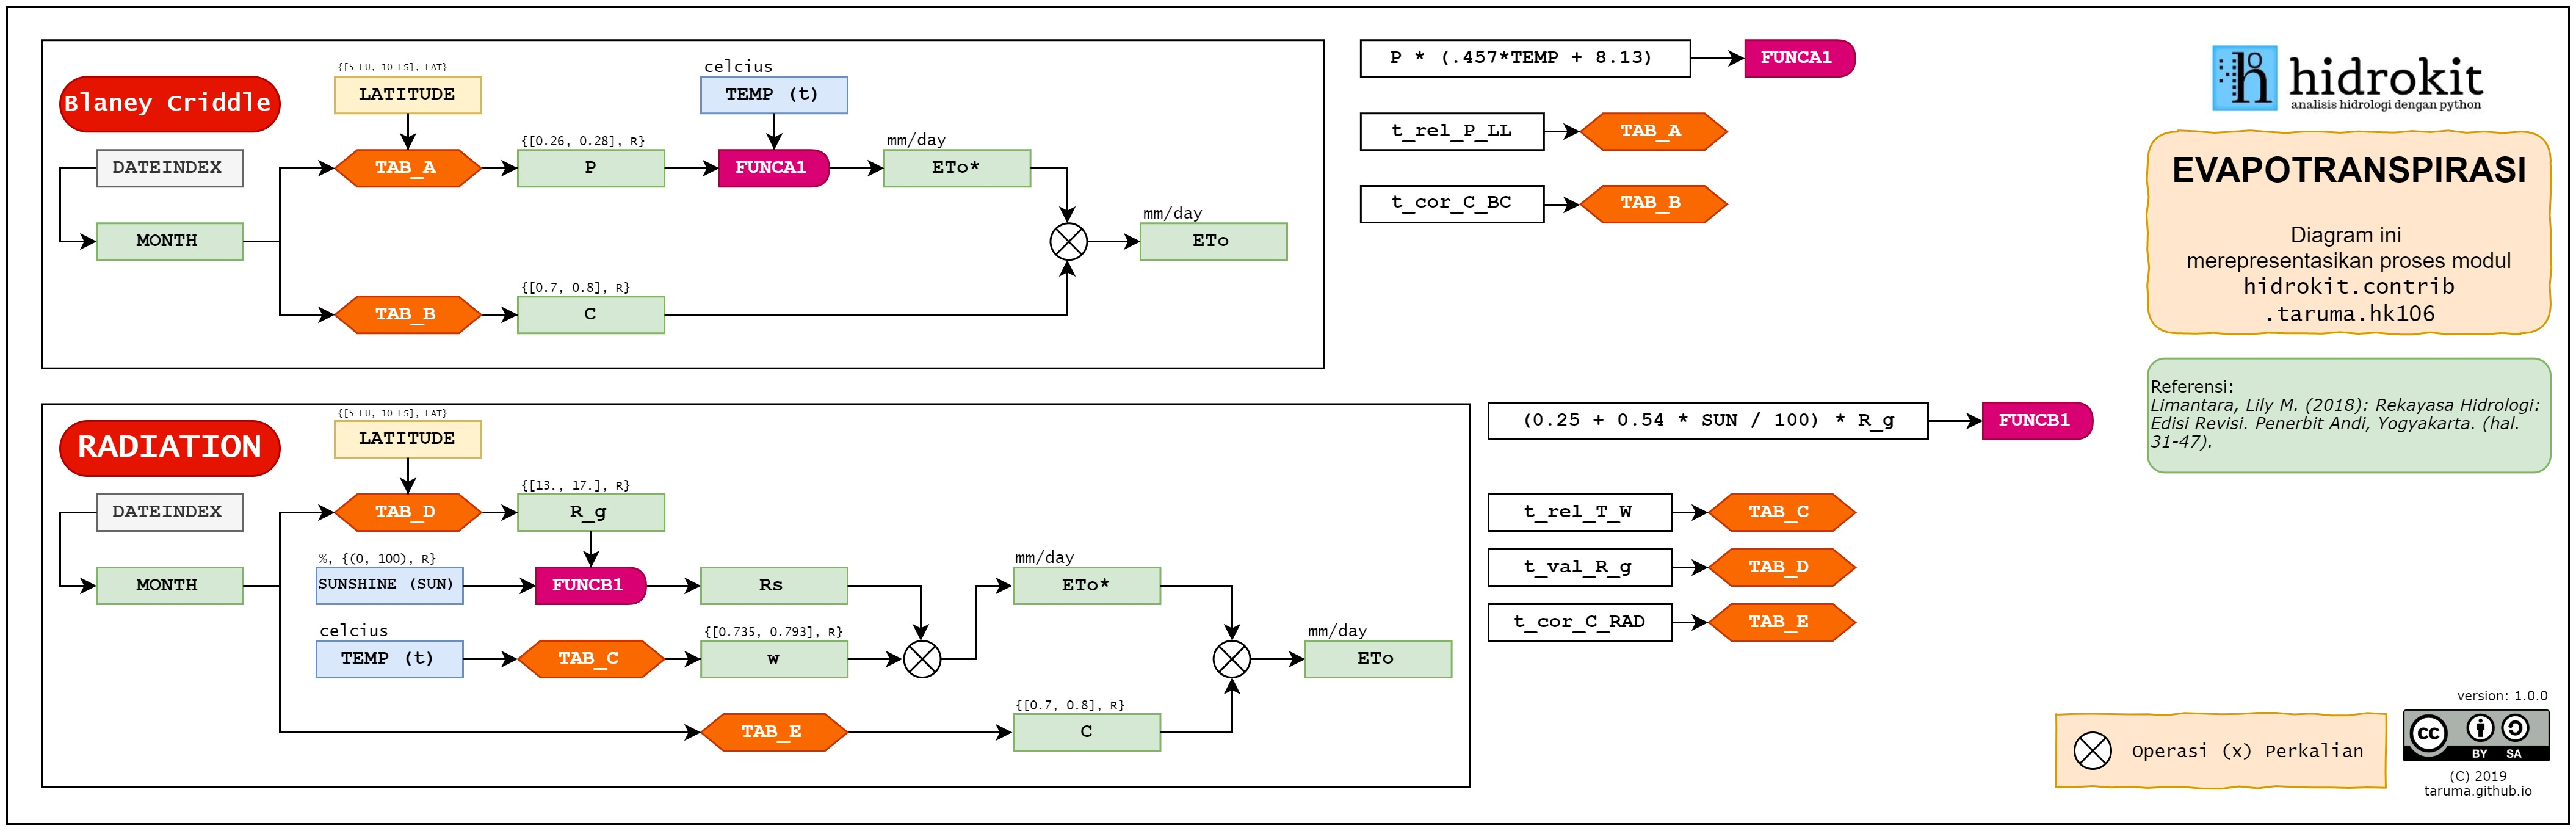
\includegraphics{https://github.com/taruma/taruma.github.io/blob/master/assets/hidrokit_assets/ETo_1_hidrokit_1_0_0.jpg?raw=true}
\caption{Blaney Criddle and Radiation Diagram}
\end{figure}

\hypertarget{diagram-rumus-penman}{%
\subsection{Diagram Rumus Penman}\label{diagram-rumus-penman}}

Diagram ini menggambarkan proses perhitungan pada fungsi
\texttt{ETo\_Penman()}

\begin{figure}
\centering
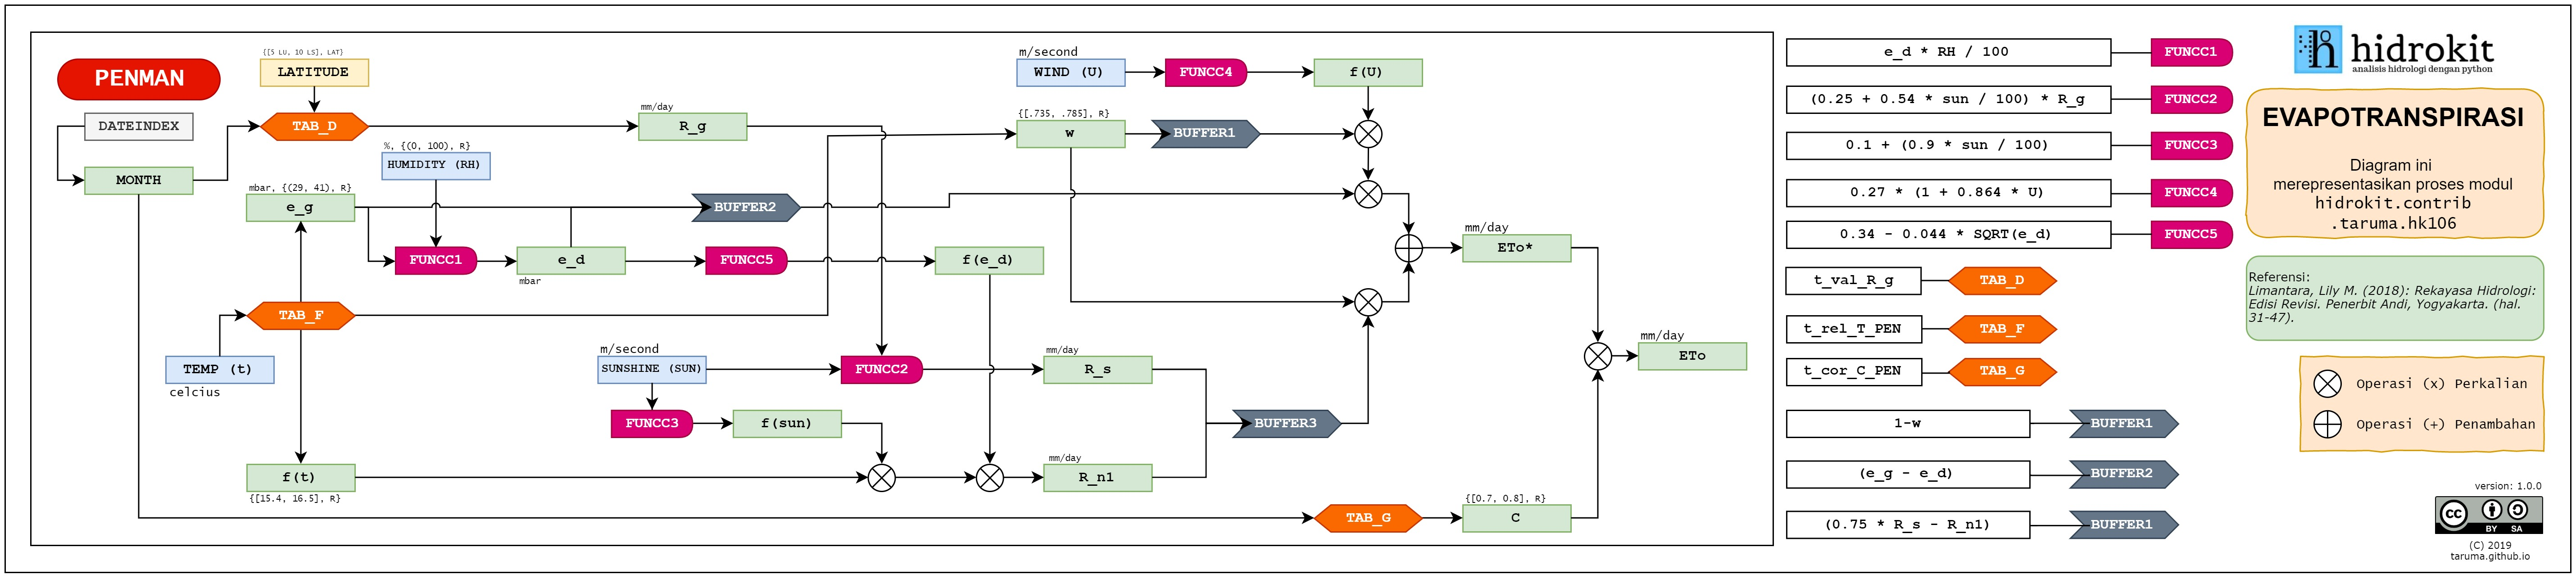
\includegraphics{https://github.com/taruma/taruma.github.io/blob/master/assets/hidrokit_assets/ETo_2_hidrokit_1_0_0.jpg?raw=true}
\caption{Blaney Criddle and Radiation Diagram}
\end{figure}

    \hypertarget{kode}{%
\section{KODE}\label{kode}}

    \begin{tcolorbox}[breakable, size=fbox, boxrule=1pt, pad at break*=1mm,colback=cellbackground, colframe=cellborder]
\prompt{In}{incolor}{ }{\boxspacing}
\begin{Verbatim}[commandchars=\\\{\}]
\PY{k}{def} \PY{n+nf}{\PYZus{}\PYZus{}lat\PYZus{}to\PYZus{}num}\PY{p}{(}\PY{n}{lat}\PY{p}{)}\PY{p}{:}
    \PY{n}{num}\PY{p}{,} \PY{n}{lat} \PY{o}{=} \PY{n}{lat}\PY{o}{.}\PY{n}{split}\PY{p}{(}\PY{l+s+s1}{\PYZsq{}}\PY{l+s+s1}{ }\PY{l+s+s1}{\PYZsq{}}\PY{p}{)}
    \PY{n}{num} \PY{o}{=} \PY{n+nb}{float}\PY{p}{(}\PY{n}{num}\PY{p}{)}
    \PY{n}{num} \PY{o}{=} \PY{o}{\PYZhy{}}\PY{n}{num} \PY{k}{if} \PY{n}{lat}\PY{o}{.}\PY{n}{lower}\PY{p}{(}\PY{p}{)} \PY{o}{==} \PY{l+s+s1}{\PYZsq{}}\PY{l+s+s1}{lu}\PY{l+s+s1}{\PYZsq{}} \PY{k}{else} \PY{n}{num}
    \PY{k}{return} \PY{n}{num}
\end{Verbatim}
\end{tcolorbox}

    \hypertarget{blaney-criddle}{%
\subsection{Blaney Criddle}\label{blaney-criddle}}

    \begin{tcolorbox}[breakable, size=fbox, boxrule=1pt, pad at break*=1mm,colback=cellbackground, colframe=cellborder]
\prompt{In}{incolor}{ }{\boxspacing}
\begin{Verbatim}[commandchars=\\\{\}]
\PY{k}{def} \PY{n+nf}{BC\PYZus{}ETo}\PY{p}{(}\PY{n}{c}\PY{p}{,} \PY{n}{ETo\PYZus{}x}\PY{p}{)}\PY{p}{:}
    \PY{k}{return} \PY{n}{c} \PY{o}{*} \PY{n}{ETo\PYZus{}x}

\PY{k}{def} \PY{n+nf}{BC\PYZus{}ETo\PYZus{}x}\PY{p}{(}\PY{n}{P}\PY{p}{,} \PY{n}{temp}\PY{p}{)}\PY{p}{:}
    \PY{k}{return} \PY{n}{P} \PY{o}{*} \PY{p}{(}\PY{l+m+mf}{.457}\PY{o}{*}\PY{n}{temp} \PY{o}{+} \PY{l+m+mf}{8.13}\PY{p}{)}

\PY{k}{def} \PY{n+nf}{BC\PYZus{}find\PYZus{}P}\PY{p}{(}\PY{n}{latitude}\PY{p}{,} \PY{n}{month}\PY{p}{,} \PY{n}{table}\PY{o}{=}\PY{n}{t\PYZus{}rel\PYZus{}P\PYZus{}LL}\PY{p}{)}\PY{p}{:}
    \PY{n}{m} \PY{o}{=} \PY{n}{table}\PY{o}{.}\PY{n}{loc}\PY{p}{[}\PY{n}{month}\PY{p}{]}\PY{o}{.}\PY{n}{values}
    \PY{n}{x} \PY{o}{=} \PY{p}{[}\PY{o}{\PYZhy{}}\PY{l+m+mi}{5}\PY{p}{,} \PY{o}{\PYZhy{}}\PY{l+m+mf}{2.5}\PY{p}{,} \PY{l+m+mi}{0}\PY{p}{,} \PY{l+m+mf}{2.5}\PY{p}{,} \PY{l+m+mi}{5}\PY{p}{,} \PY{l+m+mf}{7.5}\PY{p}{,} \PY{l+m+mi}{10}\PY{p}{]}
    \PY{k}{return} \PY{n}{np}\PY{o}{.}\PY{n}{interp}\PY{p}{(}\PY{n}{\PYZus{}\PYZus{}lat\PYZus{}to\PYZus{}num}\PY{p}{(}\PY{n}{latitude}\PY{p}{)}\PY{p}{,} \PY{n}{x}\PY{p}{,} \PY{n}{m}\PY{p}{)}

\PY{k}{def} \PY{n+nf}{BC\PYZus{}find\PYZus{}C}\PY{p}{(}\PY{n}{month}\PY{p}{,} \PY{n}{table}\PY{o}{=}\PY{n}{t\PYZus{}cor\PYZus{}C\PYZus{}BC}\PY{p}{,} \PY{n}{col}\PY{o}{=}\PY{l+s+s1}{\PYZsq{}}\PY{l+s+s1}{C}\PY{l+s+s1}{\PYZsq{}}\PY{p}{)}\PY{p}{:}
    \PY{k}{return} \PY{n}{table}\PY{o}{.}\PY{n}{loc}\PY{p}{[}\PY{n}{month}\PY{p}{,} \PY{n}{col}\PY{p}{]}
\end{Verbatim}
\end{tcolorbox}

    \begin{tcolorbox}[breakable, size=fbox, boxrule=1pt, pad at break*=1mm,colback=cellbackground, colframe=cellborder]
\prompt{In}{incolor}{ }{\boxspacing}
\begin{Verbatim}[commandchars=\\\{\}]
\PY{k}{def} \PY{n+nf}{ETo\PYZus{}BlaneyCriddle}\PY{p}{(}\PY{n}{df}\PY{p}{,} \PY{n}{temp\PYZus{}col}\PY{p}{,} \PY{n}{lat}\PY{p}{,} 
                      \PY{n}{as\PYZus{}df}\PY{o}{=}\PY{k+kc}{True}\PY{p}{,} \PY{n}{report}\PY{o}{=}\PY{l+s+s1}{\PYZsq{}}\PY{l+s+s1}{ETo}\PY{l+s+s1}{\PYZsq{}}\PY{p}{)}\PY{p}{:}

    \PY{c+c1}{\PYZsh{} sub\PYZus{}df}
    \PY{n}{data} \PY{o}{=} \PY{n}{df}\PY{o}{.}\PY{n}{loc}\PY{p}{[}\PY{p}{:}\PY{p}{,} \PY{p}{[}\PY{n}{temp\PYZus{}col}\PY{p}{]}\PY{p}{]}
    \PY{n}{data\PYZus{}array} \PY{o}{=} \PY{n}{data}\PY{o}{.}\PY{n}{values}

    \PY{c+c1}{\PYZsh{} info\PYZus{}df}
    \PY{n}{nrows} \PY{o}{=} \PY{n}{data}\PY{o}{.}\PY{n}{shape}\PY{p}{[}\PY{l+m+mi}{0}\PY{p}{]}

    \PY{c+c1}{\PYZsh{} initialization}
    \PY{p}{(}\PY{n}{P}\PY{p}{,} \PY{n}{ETo\PYZus{}x}\PY{p}{,} \PY{n}{C}\PY{p}{,} \PY{n}{ETo}\PY{p}{)} \PY{o}{=} \PY{p}{(}\PY{n}{np}\PY{o}{.}\PY{n}{zeros}\PY{p}{(}\PY{n}{nrows}\PY{p}{)} \PY{k}{for} \PY{n}{\PYZus{}} \PY{o+ow}{in} \PY{n+nb}{range}\PY{p}{(}\PY{l+m+mi}{4}\PY{p}{)}\PY{p}{)}

    \PY{c+c1}{\PYZsh{} calculation}
    \PY{n}{temp} \PY{o}{=} \PY{n}{data\PYZus{}array}\PY{p}{[}\PY{p}{:}\PY{p}{,} \PY{l+m+mi}{0}\PY{p}{]}
    \PY{n}{month} \PY{o}{=} \PY{n}{data}\PY{o}{.}\PY{n}{index}\PY{o}{.}\PY{n}{month}\PY{o}{.}\PY{n}{values}

    \PY{k}{for} \PY{n}{i} \PY{o+ow}{in} \PY{n+nb}{range}\PY{p}{(}\PY{n}{nrows}\PY{p}{)}\PY{p}{:}
        \PY{n}{P}\PY{p}{[}\PY{n}{i}\PY{p}{]}        \PY{o}{=} \PY{n}{BC\PYZus{}find\PYZus{}P}\PY{p}{(}\PY{n}{lat}\PY{p}{,} \PY{n}{month}\PY{p}{[}\PY{n}{i}\PY{p}{]}\PY{p}{)}
        \PY{n}{ETo\PYZus{}x}\PY{p}{[}\PY{n}{i}\PY{p}{]}    \PY{o}{=} \PY{n}{BC\PYZus{}ETo\PYZus{}x}\PY{p}{(}\PY{n}{P}\PY{p}{[}\PY{n}{i}\PY{p}{]}\PY{p}{,} \PY{n}{temp}\PY{p}{[}\PY{n}{i}\PY{p}{]}\PY{p}{)}
        \PY{n}{C}\PY{p}{[}\PY{n}{i}\PY{p}{]}        \PY{o}{=} \PY{n}{BC\PYZus{}find\PYZus{}C}\PY{p}{(}\PY{n}{month}\PY{p}{[}\PY{n}{i}\PY{p}{]}\PY{p}{)}
        \PY{n}{ETo}\PY{p}{[}\PY{n}{i}\PY{p}{]}      \PY{o}{=} \PY{n}{BC\PYZus{}ETo}\PY{p}{(}\PY{n}{C}\PY{p}{[}\PY{n}{i}\PY{p}{]}\PY{p}{,} \PY{n}{ETo\PYZus{}x}\PY{p}{[}\PY{n}{i}\PY{p}{]}\PY{p}{)}

    \PY{k}{if} \PY{n}{report}\PY{o}{.}\PY{n}{lower}\PY{p}{(}\PY{p}{)} \PY{o}{==} \PY{l+s+s1}{\PYZsq{}}\PY{l+s+s1}{full}\PY{l+s+s1}{\PYZsq{}}\PY{p}{:}
        \PY{n}{results} \PY{o}{=} \PY{n}{np}\PY{o}{.}\PY{n}{stack}\PY{p}{(}\PY{p}{(}
            \PY{n}{month}\PY{p}{,} \PY{n}{temp}\PY{p}{,} \PY{n}{P}\PY{p}{,} \PY{n}{ETo\PYZus{}x}\PY{p}{,} \PY{n}{C}\PY{p}{,} \PY{n}{ETo}
        \PY{p}{)}\PY{p}{,} \PY{n}{axis}\PY{o}{=}\PY{l+m+mi}{1}\PY{p}{)}
        \PY{n}{columns\PYZus{}name} \PY{o}{=} \PY{p}{[}
            \PY{l+s+s1}{\PYZsq{}}\PY{l+s+s1}{Month}\PY{l+s+s1}{\PYZsq{}}\PY{p}{,} \PY{l+s+s1}{\PYZsq{}}\PY{l+s+s1}{Temp}\PY{l+s+s1}{\PYZsq{}}\PY{p}{,} \PY{l+s+s1}{\PYZsq{}}\PY{l+s+s1}{P}\PY{l+s+s1}{\PYZsq{}}\PY{p}{,} \PY{l+s+s1}{\PYZsq{}}\PY{l+s+s1}{ETo\PYZus{}x}\PY{l+s+s1}{\PYZsq{}}\PY{p}{,} \PY{l+s+s1}{\PYZsq{}}\PY{l+s+s1}{C}\PY{l+s+s1}{\PYZsq{}}\PY{p}{,} \PY{l+s+s1}{\PYZsq{}}\PY{l+s+s1}{ETo}\PY{l+s+s1}{\PYZsq{}}
        \PY{p}{]}
    \PY{k}{elif} \PY{n}{report}\PY{o}{.}\PY{n}{lower}\PY{p}{(}\PY{p}{)} \PY{o}{==} \PY{l+s+s1}{\PYZsq{}}\PY{l+s+s1}{eto}\PY{l+s+s1}{\PYZsq{}}\PY{p}{:}
        \PY{n}{results} \PY{o}{=} \PY{n}{ETo}
        \PY{n}{columns\PYZus{}name} \PY{o}{=} \PY{p}{[}\PY{l+s+s1}{\PYZsq{}}\PY{l+s+s1}{ETo}\PY{l+s+s1}{\PYZsq{}}\PY{p}{]}
    
    \PY{k}{if} \PY{n}{as\PYZus{}df}\PY{p}{:}
        \PY{k}{return} \PY{n}{pd}\PY{o}{.}\PY{n}{DataFrame}\PY{p}{(}
            \PY{n}{data}\PY{o}{=}\PY{n}{results}\PY{p}{,} \PY{n}{index}\PY{o}{=}\PY{n}{data}\PY{o}{.}\PY{n}{index}\PY{p}{,} \PY{n}{columns}\PY{o}{=}\PY{n}{columns\PYZus{}name}
        \PY{p}{)}
    \PY{k}{else}\PY{p}{:}
        \PY{k}{return} \PY{n}{results}
\end{Verbatim}
\end{tcolorbox}

    \hypertarget{radiasi}{%
\subsection{RADIASI}\label{radiasi}}

    \begin{tcolorbox}[breakable, size=fbox, boxrule=1pt, pad at break*=1mm,colback=cellbackground, colframe=cellborder]
\prompt{In}{incolor}{ }{\boxspacing}
\begin{Verbatim}[commandchars=\\\{\}]
\PY{k}{def} \PY{n+nf}{RAD\PYZus{}ETo}\PY{p}{(}\PY{n}{C}\PY{p}{,} \PY{n}{ETo\PYZus{}x}\PY{p}{)}\PY{p}{:}
    \PY{k}{return} \PY{n}{C} \PY{o}{*} \PY{n}{ETo\PYZus{}x}

\PY{k}{def} \PY{n+nf}{RAD\PYZus{}ETo\PYZus{}x}\PY{p}{(}\PY{n}{w}\PY{p}{,} \PY{n}{Rs}\PY{p}{)}\PY{p}{:}
    \PY{k}{return} \PY{n}{w} \PY{o}{*} \PY{n}{Rs}

\PY{k}{def} \PY{n+nf}{RAD\PYZus{}find\PYZus{}W}\PY{p}{(}\PY{n}{temp}\PY{p}{,} \PY{n}{table}\PY{o}{=}\PY{n}{t\PYZus{}rel\PYZus{}T\PYZus{}W}\PY{p}{)}\PY{p}{:}
    \PY{n}{t} \PY{o}{=} \PY{n}{table}\PY{p}{[}\PY{l+s+s1}{\PYZsq{}}\PY{l+s+s1}{suhu}\PY{l+s+s1}{\PYZsq{}}\PY{p}{]}\PY{o}{.}\PY{n}{values}
    \PY{n}{w} \PY{o}{=} \PY{n}{table}\PY{p}{[}\PY{l+s+s1}{\PYZsq{}}\PY{l+s+s1}{W}\PY{l+s+s1}{\PYZsq{}}\PY{p}{]}\PY{o}{.}\PY{n}{values}
    \PY{k}{return} \PY{n}{np}\PY{o}{.}\PY{n}{interp}\PY{p}{(}\PY{n}{temp}\PY{p}{,} \PY{n}{t}\PY{p}{,} \PY{n}{w}\PY{p}{)}

\PY{k}{def} \PY{n+nf}{RAD\PYZus{}find\PYZus{}Rg}\PY{p}{(}\PY{n}{latitude}\PY{p}{,} \PY{n}{month}\PY{p}{,} \PY{n}{table}\PY{o}{=}\PY{n}{t\PYZus{}val\PYZus{}Rg}\PY{p}{)}\PY{p}{:}
    \PY{n}{m} \PY{o}{=} \PY{n}{table}\PY{o}{.}\PY{n}{loc}\PY{p}{[}\PY{n}{month}\PY{p}{]}\PY{o}{.}\PY{n}{values}
    \PY{n}{x} \PY{o}{=} \PY{p}{[}\PY{o}{\PYZhy{}}\PY{l+m+mi}{5}\PY{p}{,} \PY{o}{\PYZhy{}}\PY{l+m+mi}{4}\PY{p}{,} \PY{o}{\PYZhy{}}\PY{l+m+mi}{2}\PY{p}{,} \PY{l+m+mi}{0}\PY{p}{,} \PY{l+m+mi}{2}\PY{p}{,} \PY{l+m+mi}{4}\PY{p}{,} \PY{l+m+mi}{6}\PY{p}{,} \PY{l+m+mi}{8}\PY{p}{,} \PY{l+m+mi}{10}\PY{p}{]}
    \PY{k}{return} \PY{n}{np}\PY{o}{.}\PY{n}{interp}\PY{p}{(}\PY{n}{\PYZus{}\PYZus{}lat\PYZus{}to\PYZus{}num}\PY{p}{(}\PY{n}{latitude}\PY{p}{)}\PY{p}{,} \PY{n}{x}\PY{p}{,} \PY{n}{m}\PY{p}{)}

\PY{k}{def} \PY{n+nf}{RAD\PYZus{}Rs}\PY{p}{(}\PY{n}{sun\PYZus{}duration}\PY{p}{,} \PY{n}{Rg}\PY{p}{)}\PY{p}{:}
    \PY{k}{return} \PY{p}{(}\PY{l+m+mf}{0.25} \PY{o}{+} \PY{l+m+mf}{0.54} \PY{o}{*} \PY{n}{sun\PYZus{}duration}\PY{o}{/}\PY{l+m+mi}{100}\PY{p}{)} \PY{o}{*} \PY{n}{Rg}

\PY{k}{def} \PY{n+nf}{RAD\PYZus{}find\PYZus{}C}\PY{p}{(}\PY{n}{month}\PY{p}{,} \PY{n}{table}\PY{o}{=}\PY{n}{t\PYZus{}cor\PYZus{}C\PYZus{}RAD}\PY{p}{,} \PY{n}{col}\PY{o}{=}\PY{l+s+s1}{\PYZsq{}}\PY{l+s+s1}{C}\PY{l+s+s1}{\PYZsq{}}\PY{p}{)}\PY{p}{:}
    \PY{k}{return} \PY{n}{table}\PY{o}{.}\PY{n}{loc}\PY{p}{[}\PY{n}{month}\PY{p}{,} \PY{n}{col}\PY{p}{]}
\end{Verbatim}
\end{tcolorbox}

    \begin{tcolorbox}[breakable, size=fbox, boxrule=1pt, pad at break*=1mm,colback=cellbackground, colframe=cellborder]
\prompt{In}{incolor}{ }{\boxspacing}
\begin{Verbatim}[commandchars=\\\{\}]
\PY{k}{def} \PY{n+nf}{ETo\PYZus{}Radiation}\PY{p}{(}\PY{n}{df}\PY{p}{,} \PY{n}{temp\PYZus{}col}\PY{p}{,} \PY{n}{sun\PYZus{}col}\PY{p}{,} \PY{n}{lat}\PY{p}{,}
                  \PY{n}{as\PYZus{}df}\PY{o}{=}\PY{k+kc}{True}\PY{p}{,} \PY{n}{report}\PY{o}{=}\PY{l+s+s1}{\PYZsq{}}\PY{l+s+s1}{ETo}\PY{l+s+s1}{\PYZsq{}}\PY{p}{)}\PY{p}{:}

    \PY{c+c1}{\PYZsh{} sub\PYZus{}df}
    \PY{n}{data} \PY{o}{=} \PY{n}{df}\PY{o}{.}\PY{n}{loc}\PY{p}{[}\PY{p}{:}\PY{p}{,} \PY{p}{[}\PY{n}{temp\PYZus{}col}\PY{p}{,} \PY{n}{sun\PYZus{}col}\PY{p}{]}\PY{p}{]}
    \PY{n}{data\PYZus{}array} \PY{o}{=} \PY{n}{data}\PY{o}{.}\PY{n}{values}

    \PY{c+c1}{\PYZsh{} info\PYZus{}df}
    \PY{n}{nrows} \PY{o}{=} \PY{n}{data}\PY{o}{.}\PY{n}{shape}\PY{p}{[}\PY{l+m+mi}{0}\PY{p}{]}

    \PY{c+c1}{\PYZsh{} initialization}
    \PY{p}{(}\PY{n}{w}\PY{p}{,} \PY{n}{Rg}\PY{p}{,} \PY{n}{Rs}\PY{p}{,} \PY{n}{ETo\PYZus{}x}\PY{p}{,} \PY{n}{C}\PY{p}{,} \PY{n}{ETo}\PY{p}{)} \PY{o}{=} \PY{p}{(}\PY{n}{np}\PY{o}{.}\PY{n}{zeros}\PY{p}{(}\PY{n}{nrows}\PY{p}{)} \PY{k}{for} \PY{n}{\PYZus{}} \PY{o+ow}{in} \PY{n+nb}{range}\PY{p}{(}\PY{l+m+mi}{6}\PY{p}{)}\PY{p}{)}

    \PY{c+c1}{\PYZsh{} calculation}
    \PY{n}{temp} \PY{o}{=} \PY{n}{data\PYZus{}array}\PY{p}{[}\PY{p}{:}\PY{p}{,} \PY{l+m+mi}{0}\PY{p}{]}
    \PY{n}{sun} \PY{o}{=} \PY{n}{data\PYZus{}array}\PY{p}{[}\PY{p}{:}\PY{p}{,} \PY{l+m+mi}{1}\PY{p}{]}
    \PY{n}{month} \PY{o}{=} \PY{n}{data}\PY{o}{.}\PY{n}{index}\PY{o}{.}\PY{n}{month}\PY{o}{.}\PY{n}{values}

    \PY{k}{for} \PY{n}{i} \PY{o+ow}{in} \PY{n+nb}{range}\PY{p}{(}\PY{n}{nrows}\PY{p}{)}\PY{p}{:}
        \PY{n}{w}\PY{p}{[}\PY{n}{i}\PY{p}{]}        \PY{o}{=} \PY{n}{RAD\PYZus{}find\PYZus{}W}\PY{p}{(}\PY{n}{temp}\PY{p}{[}\PY{n}{i}\PY{p}{]}\PY{p}{)}
        \PY{n}{Rg}\PY{p}{[}\PY{n}{i}\PY{p}{]}       \PY{o}{=} \PY{n}{RAD\PYZus{}find\PYZus{}Rg}\PY{p}{(}\PY{n}{lat}\PY{p}{,} \PY{n}{month}\PY{p}{[}\PY{n}{i}\PY{p}{]}\PY{p}{)}
        \PY{n}{Rs}\PY{p}{[}\PY{n}{i}\PY{p}{]}       \PY{o}{=} \PY{n}{RAD\PYZus{}Rs}\PY{p}{(}\PY{n}{sun}\PY{p}{[}\PY{n}{i}\PY{p}{]}\PY{p}{,} \PY{n}{Rg}\PY{p}{[}\PY{n}{i}\PY{p}{]}\PY{p}{)}
        \PY{n}{ETo\PYZus{}x}\PY{p}{[}\PY{n}{i}\PY{p}{]}    \PY{o}{=} \PY{n}{RAD\PYZus{}ETo\PYZus{}x}\PY{p}{(}\PY{n}{w}\PY{p}{[}\PY{n}{i}\PY{p}{]}\PY{p}{,} \PY{n}{Rs}\PY{p}{[}\PY{n}{i}\PY{p}{]}\PY{p}{)}
        \PY{n}{C}\PY{p}{[}\PY{n}{i}\PY{p}{]}        \PY{o}{=} \PY{n}{RAD\PYZus{}find\PYZus{}C}\PY{p}{(}\PY{n}{month}\PY{p}{[}\PY{n}{i}\PY{p}{]}\PY{p}{)}
        \PY{n}{ETo}\PY{p}{[}\PY{n}{i}\PY{p}{]}      \PY{o}{=} \PY{n}{RAD\PYZus{}ETo}\PY{p}{(}\PY{n}{C}\PY{p}{[}\PY{n}{i}\PY{p}{]}\PY{p}{,} \PY{n}{ETo\PYZus{}x}\PY{p}{[}\PY{n}{i}\PY{p}{]}\PY{p}{)}


    \PY{k}{if} \PY{n}{report}\PY{o}{.}\PY{n}{lower}\PY{p}{(}\PY{p}{)} \PY{o}{==} \PY{l+s+s1}{\PYZsq{}}\PY{l+s+s1}{full}\PY{l+s+s1}{\PYZsq{}}\PY{p}{:}
        \PY{n}{results} \PY{o}{=} \PY{n}{np}\PY{o}{.}\PY{n}{stack}\PY{p}{(}\PY{p}{(}
            \PY{n}{month}\PY{p}{,} \PY{n}{temp}\PY{p}{,} \PY{n}{sun}\PY{p}{,} \PY{n}{w}\PY{p}{,} \PY{n}{Rg}\PY{p}{,} \PY{n}{Rs}\PY{p}{,} \PY{n}{ETo\PYZus{}x}\PY{p}{,} \PY{n}{C}\PY{p}{,} \PY{n}{ETo}
        \PY{p}{)}\PY{p}{,} \PY{n}{axis}\PY{o}{=}\PY{l+m+mi}{1}\PY{p}{)}
        \PY{n}{columns\PYZus{}name} \PY{o}{=} \PY{p}{[}
            \PY{l+s+s1}{\PYZsq{}}\PY{l+s+s1}{Month}\PY{l+s+s1}{\PYZsq{}}\PY{p}{,} \PY{l+s+s1}{\PYZsq{}}\PY{l+s+s1}{Temp}\PY{l+s+s1}{\PYZsq{}}\PY{p}{,} \PY{l+s+s1}{\PYZsq{}}\PY{l+s+s1}{Sun}\PY{l+s+s1}{\PYZsq{}}\PY{p}{,} \PY{l+s+s1}{\PYZsq{}}\PY{l+s+s1}{W}\PY{l+s+s1}{\PYZsq{}}\PY{p}{,} \PY{l+s+s1}{\PYZsq{}}\PY{l+s+s1}{R\PYZus{}G}\PY{l+s+s1}{\PYZsq{}}\PY{p}{,} \PY{l+s+s1}{\PYZsq{}}\PY{l+s+s1}{R\PYZus{}s}\PY{l+s+s1}{\PYZsq{}}\PY{p}{,} \PY{l+s+s1}{\PYZsq{}}\PY{l+s+s1}{ETo\PYZus{}x}\PY{l+s+s1}{\PYZsq{}}\PY{p}{,} \PY{l+s+s1}{\PYZsq{}}\PY{l+s+s1}{C}\PY{l+s+s1}{\PYZsq{}}\PY{p}{,} \PY{l+s+s1}{\PYZsq{}}\PY{l+s+s1}{ETo}\PY{l+s+s1}{\PYZsq{}}
        \PY{p}{]}
    \PY{k}{elif} \PY{n}{report}\PY{o}{.}\PY{n}{lower}\PY{p}{(}\PY{p}{)} \PY{o}{==} \PY{l+s+s1}{\PYZsq{}}\PY{l+s+s1}{eto}\PY{l+s+s1}{\PYZsq{}}\PY{p}{:}
        \PY{n}{results} \PY{o}{=} \PY{n}{ETo}
        \PY{n}{columns\PYZus{}name} \PY{o}{=} \PY{p}{[}\PY{l+s+s1}{\PYZsq{}}\PY{l+s+s1}{ETo}\PY{l+s+s1}{\PYZsq{}}\PY{p}{]}
    
    \PY{k}{if} \PY{n}{as\PYZus{}df}\PY{p}{:}
        \PY{k}{return} \PY{n}{pd}\PY{o}{.}\PY{n}{DataFrame}\PY{p}{(}
            \PY{n}{data}\PY{o}{=}\PY{n}{results}\PY{p}{,} \PY{n}{index}\PY{o}{=}\PY{n}{data}\PY{o}{.}\PY{n}{index}\PY{p}{,} \PY{n}{columns}\PY{o}{=}\PY{n}{columns\PYZus{}name}
        \PY{p}{)}
    \PY{k}{else}\PY{p}{:}
        \PY{k}{return} \PY{n}{results}
\end{Verbatim}
\end{tcolorbox}

    \hypertarget{penman}{%
\subsection{Penman}\label{penman}}

    \begin{tcolorbox}[breakable, size=fbox, boxrule=1pt, pad at break*=1mm,colback=cellbackground, colframe=cellborder]
\prompt{In}{incolor}{ }{\boxspacing}
\begin{Verbatim}[commandchars=\\\{\}]
\PY{k}{def} \PY{n+nf}{PEN\PYZus{}ETo}\PY{p}{(}\PY{n}{C}\PY{p}{,} \PY{n}{ETo\PYZus{}x}\PY{p}{)}\PY{p}{:}
    \PY{k}{return} \PY{n}{C} \PY{o}{*} \PY{n}{ETo\PYZus{}x}

\PY{k}{def} \PY{n+nf}{PEN\PYZus{}ETo\PYZus{}x}\PY{p}{(}\PY{n}{w}\PY{p}{,} \PY{n}{Rs}\PY{p}{,} \PY{n}{Rn1}\PY{p}{,} \PY{n}{fU}\PY{p}{,} \PY{n}{e\PYZus{}g}\PY{p}{,} \PY{n}{e\PYZus{}d}\PY{p}{)}\PY{p}{:}
    \PY{k}{return} \PY{n}{w} \PY{o}{*} \PY{p}{(}\PY{l+m+mf}{0.75} \PY{o}{*} \PY{n}{Rs} \PY{o}{\PYZhy{}} \PY{n}{Rn1}\PY{p}{)} \PY{o}{+} \PY{p}{(}\PY{l+m+mi}{1} \PY{o}{\PYZhy{}} \PY{n}{w}\PY{p}{)} \PY{o}{*} \PY{n}{fU} \PY{o}{*} \PY{p}{(}\PY{n}{e\PYZus{}g} \PY{o}{\PYZhy{}} \PY{n}{e\PYZus{}d}\PY{p}{)}

\PY{k}{def} \PY{n+nf}{PEN\PYZus{}Rs}\PY{p}{(}\PY{n}{sun\PYZus{}duration}\PY{p}{,} \PY{n}{RG}\PY{p}{)}\PY{p}{:}
    \PY{k}{return} \PY{p}{(}\PY{l+m+mf}{0.25} \PY{o}{+} \PY{l+m+mf}{0.54} \PY{o}{*} \PY{n}{sun\PYZus{}duration} \PY{o}{/} \PY{l+m+mi}{100}\PY{p}{)} \PY{o}{*} \PY{n}{RG}

\PY{k}{def} \PY{n+nf}{PEN\PYZus{}Rn1}\PY{p}{(}\PY{n}{ft}\PY{p}{,} \PY{n}{fe\PYZus{}d}\PY{p}{,} \PY{n}{fsun}\PY{p}{)}\PY{p}{:}
    \PY{k}{return} \PY{n}{ft} \PY{o}{*} \PY{n}{fe\PYZus{}d} \PY{o}{*} \PY{n}{fsun}

\PY{k}{def} \PY{n+nf}{PEN\PYZus{}fe\PYZus{}d}\PY{p}{(}\PY{n}{e\PYZus{}d}\PY{p}{)}\PY{p}{:}
    \PY{k}{return} \PY{l+m+mf}{0.34} \PY{o}{\PYZhy{}} \PY{l+m+mf}{0.044} \PY{o}{*} \PY{n}{np}\PY{o}{.}\PY{n}{sqrt}\PY{p}{(}\PY{n}{e\PYZus{}d}\PY{p}{)}

\PY{k}{def} \PY{n+nf}{PEN\PYZus{}e\PYZus{}d}\PY{p}{(}\PY{n}{e\PYZus{}d}\PY{p}{,} \PY{n}{RH}\PY{p}{)}\PY{p}{:}
    \PY{k}{return} \PY{n}{e\PYZus{}d} \PY{o}{*} \PY{n}{RH} \PY{o}{/}\PY{l+m+mi}{100}

\PY{k}{def} \PY{n+nf}{PEN\PYZus{}fsun}\PY{p}{(}\PY{n}{sun\PYZus{}duration}\PY{p}{)}\PY{p}{:}
    \PY{k}{return} \PY{l+m+mf}{0.1} \PY{o}{+} \PY{p}{(}\PY{l+m+mf}{0.9} \PY{o}{*} \PY{n}{sun\PYZus{}duration} \PY{o}{/} \PY{l+m+mi}{100}\PY{p}{)}

\PY{k}{def} \PY{n+nf}{PEN\PYZus{}fU}\PY{p}{(}\PY{n}{U}\PY{p}{)}\PY{p}{:}
    \PY{k}{return} \PY{l+m+mf}{0.27} \PY{o}{*} \PY{p}{(}\PY{l+m+mi}{1} \PY{o}{+} \PY{l+m+mf}{0.864} \PY{o}{*} \PY{n}{U}\PY{p}{)}

\PY{k}{def} \PY{n+nf}{PEN\PYZus{}find\PYZus{}from\PYZus{}T}\PY{p}{(}\PY{n}{temp}\PY{p}{,} \PY{n}{table}\PY{o}{=}\PY{n}{t\PYZus{}rel\PYZus{}T\PYZus{}PEN}\PY{p}{)}\PY{p}{:}
    \PY{n}{t} \PY{o}{=} \PY{n}{table}\PY{p}{[}\PY{l+s+s1}{\PYZsq{}}\PY{l+s+s1}{suhu}\PY{l+s+s1}{\PYZsq{}}\PY{p}{]}\PY{o}{.}\PY{n}{values}
    \PY{n}{e} \PY{o}{=} \PY{n}{table}\PY{p}{[}\PY{l+s+s1}{\PYZsq{}}\PY{l+s+s1}{e\PYZus{}mbar}\PY{l+s+s1}{\PYZsq{}}\PY{p}{]}\PY{o}{.}\PY{n}{values}
    \PY{n}{w} \PY{o}{=} \PY{n}{table}\PY{p}{[}\PY{l+s+s1}{\PYZsq{}}\PY{l+s+s1}{w}\PY{l+s+s1}{\PYZsq{}}\PY{p}{]}\PY{o}{.}\PY{n}{values}
    \PY{n}{ft} \PY{o}{=} \PY{n}{table}\PY{p}{[}\PY{l+s+s1}{\PYZsq{}}\PY{l+s+s1}{f\PYZus{}t}\PY{l+s+s1}{\PYZsq{}}\PY{p}{]}\PY{o}{.}\PY{n}{values}

    \PY{k}{return} \PY{p}{(}
        \PY{n}{np}\PY{o}{.}\PY{n}{interp}\PY{p}{(}\PY{n}{temp}\PY{p}{,} \PY{n}{t}\PY{p}{,} \PY{n}{e}\PY{p}{)}\PY{p}{,}
        \PY{n}{np}\PY{o}{.}\PY{n}{interp}\PY{p}{(}\PY{n}{temp}\PY{p}{,} \PY{n}{t}\PY{p}{,} \PY{n}{w}\PY{p}{)}\PY{p}{,}
        \PY{n}{np}\PY{o}{.}\PY{n}{interp}\PY{p}{(}\PY{n}{temp}\PY{p}{,} \PY{n}{t}\PY{p}{,} \PY{n}{ft}\PY{p}{)}
    \PY{p}{)}

\PY{k}{def} \PY{n+nf}{PEN\PYZus{}find\PYZus{}Rg}\PY{p}{(}\PY{n}{latitude}\PY{p}{,} \PY{n}{month}\PY{p}{,} \PY{n}{table}\PY{o}{=}\PY{n}{t\PYZus{}val\PYZus{}Rg}\PY{p}{)}\PY{p}{:}
    \PY{n}{m} \PY{o}{=} \PY{n}{table}\PY{o}{.}\PY{n}{loc}\PY{p}{[}\PY{n}{month}\PY{p}{]}\PY{o}{.}\PY{n}{values}
    \PY{n}{x} \PY{o}{=} \PY{p}{[}\PY{o}{\PYZhy{}}\PY{l+m+mi}{5}\PY{p}{,} \PY{o}{\PYZhy{}}\PY{l+m+mi}{4}\PY{p}{,} \PY{o}{\PYZhy{}}\PY{l+m+mi}{2}\PY{p}{,} \PY{l+m+mi}{0}\PY{p}{,} \PY{l+m+mi}{2}\PY{p}{,} \PY{l+m+mi}{4}\PY{p}{,} \PY{l+m+mi}{6}\PY{p}{,} \PY{l+m+mi}{8}\PY{p}{,} \PY{l+m+mi}{10}\PY{p}{]}
    \PY{k}{return} \PY{n}{np}\PY{o}{.}\PY{n}{interp}\PY{p}{(}\PY{n}{\PYZus{}\PYZus{}lat\PYZus{}to\PYZus{}num}\PY{p}{(}\PY{n}{latitude}\PY{p}{)}\PY{p}{,} \PY{n}{x}\PY{p}{,} \PY{n}{m}\PY{p}{)}

\PY{k}{def} \PY{n+nf}{PEN\PYZus{}find\PYZus{}C}\PY{p}{(}\PY{n}{month}\PY{p}{,} \PY{n}{table}\PY{o}{=}\PY{n}{t\PYZus{}cor\PYZus{}C\PYZus{}PEN}\PY{p}{,} \PY{n}{col}\PY{o}{=}\PY{l+s+s1}{\PYZsq{}}\PY{l+s+s1}{C}\PY{l+s+s1}{\PYZsq{}}\PY{p}{)}\PY{p}{:}
    \PY{k}{return} \PY{n}{table}\PY{o}{.}\PY{n}{loc}\PY{p}{[}\PY{n}{month}\PY{p}{,} \PY{n}{col}\PY{p}{]}
\end{Verbatim}
\end{tcolorbox}

    \begin{tcolorbox}[breakable, size=fbox, boxrule=1pt, pad at break*=1mm,colback=cellbackground, colframe=cellborder]
\prompt{In}{incolor}{ }{\boxspacing}
\begin{Verbatim}[commandchars=\\\{\}]
\PY{k}{def} \PY{n+nf}{ETo\PYZus{}Penman}\PY{p}{(}\PY{n}{df}\PY{p}{,} \PY{n}{temp\PYZus{}col}\PY{p}{,} \PY{n}{humid\PYZus{}col}\PY{p}{,} \PY{n}{wind\PYZus{}col}\PY{p}{,} \PY{n}{sun\PYZus{}col}\PY{p}{,} \PY{n}{lat}\PY{p}{,}
               \PY{n}{as\PYZus{}df}\PY{o}{=}\PY{k+kc}{True}\PY{p}{,} \PY{n}{report}\PY{o}{=}\PY{l+s+s1}{\PYZsq{}}\PY{l+s+s1}{ETo}\PY{l+s+s1}{\PYZsq{}}\PY{p}{)}\PY{p}{:}

    \PY{c+c1}{\PYZsh{} sub\PYZus{}df}
    \PY{n}{data} \PY{o}{=} \PY{n}{df}\PY{o}{.}\PY{n}{loc}\PY{p}{[}\PY{p}{:}\PY{p}{,} \PY{p}{[}\PY{n}{temp\PYZus{}col}\PY{p}{,} \PY{n}{humid\PYZus{}col}\PY{p}{,} \PY{n}{wind\PYZus{}col}\PY{p}{,} \PY{n}{sun\PYZus{}col}\PY{p}{]}\PY{p}{]}
    \PY{n}{data\PYZus{}array} \PY{o}{=} \PY{n}{data}\PY{o}{.}\PY{n}{values}

    \PY{c+c1}{\PYZsh{} info\PYZus{}df}
    \PY{n}{nrows} \PY{o}{=} \PY{n}{data}\PY{o}{.}\PY{n}{shape}\PY{p}{[}\PY{l+m+mi}{0}\PY{p}{]}

    \PY{c+c1}{\PYZsh{} initialization}
    \PY{p}{(}\PY{n}{e\PYZus{}g}\PY{p}{,} \PY{n}{w}\PY{p}{,} \PY{n}{ft}\PY{p}{,} \PY{n}{fed}\PY{p}{,} \PY{n}{e\PYZus{}d}\PY{p}{,} \PY{n}{Rg}\PY{p}{,} \PY{n}{Rs}\PY{p}{,} \PY{n}{fsun}\PY{p}{,}
     \PY{n}{fU}\PY{p}{,} \PY{n}{Rn1}\PY{p}{,} \PY{n}{C}\PY{p}{,} \PY{n}{ETo\PYZus{}x}\PY{p}{,} \PY{n}{ETo}\PY{p}{)} \PY{o}{=} \PY{p}{(}\PY{n}{np}\PY{o}{.}\PY{n}{zeros}\PY{p}{(}\PY{n}{nrows}\PY{p}{)} \PY{k}{for} \PY{n}{\PYZus{}} \PY{o+ow}{in} \PY{n+nb}{range}\PY{p}{(}\PY{l+m+mi}{13}\PY{p}{)}\PY{p}{)}

    \PY{c+c1}{\PYZsh{} calculation}
    \PY{n}{temp} \PY{o}{=} \PY{n}{data\PYZus{}array}\PY{p}{[}\PY{p}{:}\PY{p}{,} \PY{l+m+mi}{0}\PY{p}{]}
    \PY{n}{RH} \PY{o}{=} \PY{n}{data\PYZus{}array}\PY{p}{[}\PY{p}{:}\PY{p}{,} \PY{l+m+mi}{1}\PY{p}{]}
    \PY{n}{wind} \PY{o}{=} \PY{n}{data\PYZus{}array}\PY{p}{[}\PY{p}{:}\PY{p}{,} \PY{l+m+mi}{2}\PY{p}{]}
    \PY{n}{sun} \PY{o}{=} \PY{n}{data\PYZus{}array}\PY{p}{[}\PY{p}{:}\PY{p}{,} \PY{l+m+mi}{3}\PY{p}{]}
    \PY{n}{month} \PY{o}{=} \PY{n}{data}\PY{o}{.}\PY{n}{index}\PY{o}{.}\PY{n}{month}\PY{o}{.}\PY{n}{values}

    \PY{k}{for} \PY{n}{i} \PY{o+ow}{in} \PY{n+nb}{range}\PY{p}{(}\PY{n}{nrows}\PY{p}{)}\PY{p}{:}
        \PY{n}{e\PYZus{}g}\PY{p}{[}\PY{n}{i}\PY{p}{]}\PY{p}{,} \PY{n}{w}\PY{p}{[}\PY{n}{i}\PY{p}{]}\PY{p}{,} \PY{n}{ft}\PY{p}{[}\PY{n}{i}\PY{p}{]} \PY{o}{=} \PY{n}{PEN\PYZus{}find\PYZus{}from\PYZus{}T}\PY{p}{(}\PY{n}{temp}\PY{p}{[}\PY{n}{i}\PY{p}{]}\PY{p}{)}
        \PY{n}{e\PYZus{}d}\PY{p}{[}\PY{n}{i}\PY{p}{]}      \PY{o}{=} \PY{n}{PEN\PYZus{}e\PYZus{}d}\PY{p}{(}\PY{n}{e\PYZus{}g}\PY{p}{[}\PY{n}{i}\PY{p}{]}\PY{p}{,} \PY{n}{RH}\PY{p}{[}\PY{n}{i}\PY{p}{]}\PY{p}{)}
        \PY{n}{fed}\PY{p}{[}\PY{n}{i}\PY{p}{]}      \PY{o}{=} \PY{n}{PEN\PYZus{}fe\PYZus{}d}\PY{p}{(}\PY{n}{e\PYZus{}d}\PY{p}{[}\PY{n}{i}\PY{p}{]}\PY{p}{)}
        \PY{n}{Rg}\PY{p}{[}\PY{n}{i}\PY{p}{]}       \PY{o}{=} \PY{n}{PEN\PYZus{}find\PYZus{}Rg}\PY{p}{(}\PY{n}{lat}\PY{p}{,} \PY{n}{month}\PY{p}{[}\PY{n}{i}\PY{p}{]}\PY{p}{)}
        \PY{n}{Rs}\PY{p}{[}\PY{n}{i}\PY{p}{]}       \PY{o}{=} \PY{n}{PEN\PYZus{}Rs}\PY{p}{(}\PY{n}{sun}\PY{p}{[}\PY{n}{i}\PY{p}{]}\PY{p}{,} \PY{n}{Rg}\PY{p}{[}\PY{n}{i}\PY{p}{]}\PY{p}{)}
        \PY{n}{fsun}\PY{p}{[}\PY{n}{i}\PY{p}{]}     \PY{o}{=} \PY{n}{PEN\PYZus{}fsun}\PY{p}{(}\PY{n}{sun}\PY{p}{[}\PY{n}{i}\PY{p}{]}\PY{p}{)}
        \PY{n}{fU}\PY{p}{[}\PY{n}{i}\PY{p}{]}       \PY{o}{=} \PY{n}{PEN\PYZus{}fU}\PY{p}{(}\PY{n}{wind}\PY{p}{[}\PY{n}{i}\PY{p}{]}\PY{p}{)}
        \PY{n}{Rn1}\PY{p}{[}\PY{n}{i}\PY{p}{]}      \PY{o}{=} \PY{n}{PEN\PYZus{}Rn1}\PY{p}{(}\PY{n}{ft}\PY{p}{[}\PY{n}{i}\PY{p}{]}\PY{p}{,} \PY{n}{fed}\PY{p}{[}\PY{n}{i}\PY{p}{]}\PY{p}{,} \PY{n}{fsun}\PY{p}{[}\PY{n}{i}\PY{p}{]}\PY{p}{)}
        \PY{n}{C}\PY{p}{[}\PY{n}{i}\PY{p}{]}        \PY{o}{=} \PY{n}{PEN\PYZus{}find\PYZus{}C}\PY{p}{(}\PY{n}{month}\PY{p}{[}\PY{n}{i}\PY{p}{]}\PY{p}{)}
        \PY{n}{ETo\PYZus{}x}\PY{p}{[}\PY{n}{i}\PY{p}{]}    \PY{o}{=} \PY{n}{PEN\PYZus{}ETo\PYZus{}x}\PY{p}{(}\PY{n}{w}\PY{p}{[}\PY{n}{i}\PY{p}{]}\PY{p}{,} \PY{n}{Rs}\PY{p}{[}\PY{n}{i}\PY{p}{]}\PY{p}{,} \PY{n}{Rn1}\PY{p}{[}\PY{n}{i}\PY{p}{]}\PY{p}{,} \PY{n}{fU}\PY{p}{[}\PY{n}{i}\PY{p}{]}\PY{p}{,} \PY{n}{e\PYZus{}g}\PY{p}{[}\PY{n}{i}\PY{p}{]}\PY{p}{,} \PY{n}{e\PYZus{}d}\PY{p}{[}\PY{n}{i}\PY{p}{]}\PY{p}{)}
        \PY{n}{ETo}\PY{p}{[}\PY{n}{i}\PY{p}{]}      \PY{o}{=} \PY{n}{PEN\PYZus{}ETo}\PY{p}{(}\PY{n}{C}\PY{p}{[}\PY{n}{i}\PY{p}{]}\PY{p}{,} \PY{n}{ETo\PYZus{}x}\PY{p}{[}\PY{n}{i}\PY{p}{]}\PY{p}{)}


    \PY{k}{if} \PY{n}{report}\PY{o}{.}\PY{n}{lower}\PY{p}{(}\PY{p}{)} \PY{o}{==} \PY{l+s+s1}{\PYZsq{}}\PY{l+s+s1}{full}\PY{l+s+s1}{\PYZsq{}}\PY{p}{:}
        \PY{n}{results} \PY{o}{=} \PY{n}{np}\PY{o}{.}\PY{n}{stack}\PY{p}{(}\PY{p}{(}
            \PY{n}{month}\PY{p}{,} \PY{n}{temp}\PY{p}{,} \PY{n}{RH}\PY{p}{,} \PY{n}{wind}\PY{p}{,} \PY{n}{sun}\PY{p}{,} \PY{n}{e\PYZus{}g}\PY{p}{,} \PY{n}{w}\PY{p}{,} \PY{n}{ft}\PY{p}{,} \PY{n}{e\PYZus{}d}\PY{p}{,} \PY{n}{fed}\PY{p}{,} \PY{n}{Rg}\PY{p}{,} \PY{n}{Rs}\PY{p}{,}
            \PY{n}{fsun}\PY{p}{,} \PY{n}{fU}\PY{p}{,} \PY{n}{Rn1}\PY{p}{,} \PY{n}{C}\PY{p}{,} \PY{n}{ETo\PYZus{}x}\PY{p}{,} \PY{n}{ETo}
        \PY{p}{)}\PY{p}{,} \PY{n}{axis}\PY{o}{=}\PY{l+m+mi}{1}\PY{p}{)}
        \PY{n}{columns\PYZus{}name} \PY{o}{=} \PY{p}{[}
            \PY{l+s+s1}{\PYZsq{}}\PY{l+s+s1}{Month}\PY{l+s+s1}{\PYZsq{}}\PY{p}{,} \PY{l+s+s1}{\PYZsq{}}\PY{l+s+s1}{Temp}\PY{l+s+s1}{\PYZsq{}}\PY{p}{,} \PY{l+s+s1}{\PYZsq{}}\PY{l+s+s1}{Humidity}\PY{l+s+s1}{\PYZsq{}}\PY{p}{,} \PY{l+s+s1}{\PYZsq{}}\PY{l+s+s1}{Wind}\PY{l+s+s1}{\PYZsq{}}\PY{p}{,} \PY{l+s+s1}{\PYZsq{}}\PY{l+s+s1}{Sun}\PY{l+s+s1}{\PYZsq{}}\PY{p}{,} \PY{l+s+s1}{\PYZsq{}}\PY{l+s+s1}{e\PYZus{}g}\PY{l+s+s1}{\PYZsq{}}\PY{p}{,} \PY{l+s+s1}{\PYZsq{}}\PY{l+s+s1}{w}\PY{l+s+s1}{\PYZsq{}}\PY{p}{,} \PY{l+s+s1}{\PYZsq{}}\PY{l+s+s1}{f\PYZus{}t}\PY{l+s+s1}{\PYZsq{}}\PY{p}{,}
            \PY{l+s+s1}{\PYZsq{}}\PY{l+s+s1}{e\PYZus{}d}\PY{l+s+s1}{\PYZsq{}}\PY{p}{,} \PY{l+s+s1}{\PYZsq{}}\PY{l+s+s1}{f\PYZus{}e\PYZus{}d}\PY{l+s+s1}{\PYZsq{}}\PY{p}{,} \PY{l+s+s1}{\PYZsq{}}\PY{l+s+s1}{R\PYZus{}g}\PY{l+s+s1}{\PYZsq{}}\PY{p}{,} \PY{l+s+s1}{\PYZsq{}}\PY{l+s+s1}{R\PYZus{}s}\PY{l+s+s1}{\PYZsq{}}\PY{p}{,} \PY{l+s+s1}{\PYZsq{}}\PY{l+s+s1}{f\PYZus{}sun}\PY{l+s+s1}{\PYZsq{}}\PY{p}{,} \PY{l+s+s1}{\PYZsq{}}\PY{l+s+s1}{f\PYZus{}U}\PY{l+s+s1}{\PYZsq{}}\PY{p}{,} \PY{l+s+s1}{\PYZsq{}}\PY{l+s+s1}{R\PYZus{}n1}\PY{l+s+s1}{\PYZsq{}}\PY{p}{,} \PY{l+s+s1}{\PYZsq{}}\PY{l+s+s1}{C}\PY{l+s+s1}{\PYZsq{}}\PY{p}{,} \PY{l+s+s1}{\PYZsq{}}\PY{l+s+s1}{ETo\PYZus{}x}\PY{l+s+s1}{\PYZsq{}}\PY{p}{,}
            \PY{l+s+s1}{\PYZsq{}}\PY{l+s+s1}{ETo}\PY{l+s+s1}{\PYZsq{}}
        \PY{p}{]}
    \PY{k}{elif} \PY{n}{report}\PY{o}{.}\PY{n}{lower}\PY{p}{(}\PY{p}{)} \PY{o}{==} \PY{l+s+s1}{\PYZsq{}}\PY{l+s+s1}{eto}\PY{l+s+s1}{\PYZsq{}}\PY{p}{:}
        \PY{n}{results} \PY{o}{=} \PY{n}{ETo}
        \PY{n}{columns\PYZus{}name} \PY{o}{=} \PY{p}{[}\PY{l+s+s1}{\PYZsq{}}\PY{l+s+s1}{ETo}\PY{l+s+s1}{\PYZsq{}}\PY{p}{]}
    
    \PY{k}{if} \PY{n}{as\PYZus{}df}\PY{p}{:}
        \PY{k}{return} \PY{n}{pd}\PY{o}{.}\PY{n}{DataFrame}\PY{p}{(}
            \PY{n}{data}\PY{o}{=}\PY{n}{results}\PY{p}{,} \PY{n}{index}\PY{o}{=}\PY{n}{data}\PY{o}{.}\PY{n}{index}\PY{p}{,} \PY{n}{columns}\PY{o}{=}\PY{n}{columns\PYZus{}name}
        \PY{p}{)}
    \PY{k}{else}\PY{p}{:}
        \PY{k}{return} \PY{n}{results}
\end{Verbatim}
\end{tcolorbox}

    \hypertarget{fungsi}{%
\section{FUNGSI}\label{fungsi}}

Dalam modul ini terdapat tiga fungsi utama yang memiliki rumus berbeda
yaitu \texttt{ETo\_BlaneyCriddle()} untuk rumus Blaney Criddle,
\texttt{ETo\_Radiation()} untuk rumus Radiasi, \texttt{ETo\_Penman()}
untuk rumus Penman.

Ketiga ini memiliki keserupaan argumen dalam fungsi, berikut argumen
yang terdapat pada ketiga fungsi: - \texttt{df}: dataset objek
\texttt{pandas.DataFrame} dengan index berupa objek
\texttt{DatetimeIndex} atau yang serupa. - \texttt{lat}: posisi lintang
lokasi dalam bentuk \emph{string} seperti
\texttt{5\ LU}/\texttt{3.5\ LS}. - (opsional) \texttt{as\_df=True}
(\emph{default}), keluaran berupa \texttt{pandas.DataFrame}. Keluaran
berupa \texttt{numpy.ndarray} jika \texttt{False}. - (opsional)
\texttt{report=\textquotesingle{}ETo\textquotesingle{}}
(\emph{default}), terdapat beberapa nilai yang dapat diterima oleh
argumen \texttt{report}: - \texttt{full}: keluaran akan menyertakan
seluruh peubah yang dihitung dalam model. - \texttt{Eto}: keluaran hanya
menyertakan kolom \texttt{ETo} (hasil akhir model).

    \hypertarget{fungsi-eto_blaneycriddle}{%
\subsection{\texorpdfstring{Fungsi
\texttt{ETo\_BlaneyCriddle()}}{Fungsi ETo\_BlaneyCriddle()}}\label{fungsi-eto_blaneycriddle}}

Selain argumen posisi \texttt{df}, \texttt{lat} dan argumen opsional
\texttt{as\_df}, \texttt{report}, fungsi ini membutuhkan argumen
\texttt{temp\_col} yaitu nama kolom suhu.

    \begin{tcolorbox}[breakable, size=fbox, boxrule=1pt, pad at break*=1mm,colback=cellbackground, colframe=cellborder]
\prompt{In}{incolor}{ }{\boxspacing}
\begin{Verbatim}[commandchars=\\\{\}]
\PY{n}{sample} \PY{o}{=} \PY{n}{pd}\PY{o}{.}\PY{n}{DataFrame}\PY{p}{(}
    \PY{n}{data}\PY{o}{=}\PY{p}{[}\PY{l+m+mf}{27.2}\PY{p}{,}\PY{l+m+mf}{27.4}\PY{p}{,}\PY{l+m+mf}{27.3}\PY{p}{,}\PY{l+m+mf}{27.9}\PY{p}{,}\PY{l+m+mf}{27.9}\PY{p}{,}\PY{l+m+mf}{26.8}\PY{p}{,}\PY{l+m+mf}{26.9}\PY{p}{,}\PY{l+m+mf}{28.6}\PY{p}{,}\PY{l+m+mf}{27.9}\PY{p}{,}\PY{l+m+mf}{27.5}\PY{p}{,}\PY{l+m+mf}{27.7}\PY{p}{,}\PY{l+m+mf}{27.3}\PY{p}{]}\PY{p}{,}
    \PY{n}{index}\PY{o}{=}\PY{n}{pd}\PY{o}{.}\PY{n}{date\PYZus{}range}\PY{p}{(}\PY{l+s+s1}{\PYZsq{}}\PY{l+s+s1}{20010101}\PY{l+s+s1}{\PYZsq{}}\PY{p}{,} \PY{n}{periods}\PY{o}{=}\PY{l+m+mi}{12}\PY{p}{,} \PY{n}{freq}\PY{o}{=}\PY{l+s+s1}{\PYZsq{}}\PY{l+s+s1}{MS}\PY{l+s+s1}{\PYZsq{}}\PY{p}{)}\PY{p}{,}
    \PY{n}{columns}\PY{o}{=}\PY{p}{[}\PY{l+s+s1}{\PYZsq{}}\PY{l+s+s1}{temp\PYZus{}C}\PY{l+s+s1}{\PYZsq{}}\PY{p}{]}
\PY{p}{)}
\end{Verbatim}
\end{tcolorbox}

    \hypertarget{default-as_dffalse}{%
\subsubsection{\texorpdfstring{default,
\texttt{as\_df=False}}{default, as\_df=False}}\label{default-as_dffalse}}

    \begin{tcolorbox}[breakable, size=fbox, boxrule=1pt, pad at break*=1mm,colback=cellbackground, colframe=cellborder]
\prompt{In}{incolor}{ }{\boxspacing}
\begin{Verbatim}[commandchars=\\\{\}]
\PY{n}{ETo\PYZus{}BlaneyCriddle}\PY{p}{(}\PY{n}{df}\PY{o}{=}\PY{n}{sample}\PY{p}{,} 
                  \PY{n}{temp\PYZus{}col}\PY{o}{=}\PY{l+s+s1}{\PYZsq{}}\PY{l+s+s1}{temp\PYZus{}C}\PY{l+s+s1}{\PYZsq{}}\PY{p}{,} 
                  \PY{n}{lat}\PY{o}{=}\PY{l+s+s1}{\PYZsq{}}\PY{l+s+s1}{7.5 LS}\PY{l+s+s1}{\PYZsq{}}\PY{p}{,}
                  \PY{n}{as\PYZus{}df}\PY{o}{=}\PY{k+kc}{False}\PY{p}{)}
\end{Verbatim}
\end{tcolorbox}

            \begin{tcolorbox}[breakable, size=fbox, boxrule=.5pt, pad at break*=1mm, opacityfill=0]
\prompt{Out}{outcolor}{ }{\boxspacing}
\begin{Verbatim}[commandchars=\\\{\}]
array([4.6055296, 4.6260032, 4.327281 , 4.0925388, 3.9463767, 3.8513664,
       3.8600037, 4.2930405, 4.6771872, 4.63624  , 4.6567136, 4.7806152])
\end{Verbatim}
\end{tcolorbox}
        
    \hypertarget{reportfull}{%
\subsubsection{\texorpdfstring{\texttt{report=\textquotesingle{}full\textquotesingle{}}}{report='full'}}\label{reportfull}}

    \begin{tcolorbox}[breakable, size=fbox, boxrule=1pt, pad at break*=1mm,colback=cellbackground, colframe=cellborder]
\prompt{In}{incolor}{ }{\boxspacing}
\begin{Verbatim}[commandchars=\\\{\}]
\PY{n}{ETo\PYZus{}BlaneyCriddle}\PY{p}{(}\PY{n}{df}\PY{o}{=}\PY{n}{sample}\PY{p}{,} 
                  \PY{n}{temp\PYZus{}col}\PY{o}{=}\PY{l+s+s1}{\PYZsq{}}\PY{l+s+s1}{temp\PYZus{}C}\PY{l+s+s1}{\PYZsq{}}\PY{p}{,} 
                  \PY{n}{lat}\PY{o}{=}\PY{l+s+s1}{\PYZsq{}}\PY{l+s+s1}{7.5 LS}\PY{l+s+s1}{\PYZsq{}}\PY{p}{,}
                  \PY{n}{report}\PY{o}{=}\PY{l+s+s1}{\PYZsq{}}\PY{l+s+s1}{full}\PY{l+s+s1}{\PYZsq{}}\PY{p}{)}
\end{Verbatim}
\end{tcolorbox}

            \begin{tcolorbox}[breakable, size=fbox, boxrule=.5pt, pad at break*=1mm, opacityfill=0]
\prompt{Out}{outcolor}{ }{\boxspacing}
\begin{Verbatim}[commandchars=\\\{\}]
            Month  Temp     P     ETo\_x     C       ETo
2001-01-01    1.0  27.2  0.28  5.756912  0.80  4.605530
2001-02-01    2.0  27.4  0.28  5.782504  0.80  4.626003
2001-03-01    3.0  27.3  0.28  5.769708  0.75  4.327281
2001-04-01    4.0  27.9  0.28  5.846484  0.70  4.092539
2001-05-01    5.0  27.9  0.27  5.637681  0.70  3.946377
2001-06-01    6.0  26.8  0.27  5.501952  0.70  3.851366
2001-07-01    7.0  26.9  0.27  5.514291  0.70  3.860004
2001-08-01    8.0  28.6  0.27  5.724054  0.75  4.293041
2001-09-01    9.0  27.9  0.28  5.846484  0.80  4.677187
2001-10-01   10.0  27.5  0.28  5.795300  0.80  4.636240
2001-11-01   11.0  27.7  0.28  5.820892  0.80  4.656714
2001-12-01   12.0  27.3  0.29  5.975769  0.80  4.780615
\end{Verbatim}
\end{tcolorbox}
        
    \hypertarget{fungsi-eto_radiation}{%
\subsection{\texorpdfstring{Fungsi
\texttt{ETo\_Radiation()}}{Fungsi ETo\_Radiation()}}\label{fungsi-eto_radiation}}

Selain argumen posisi \texttt{df}, \texttt{lat} dan argumen opsional
\texttt{as\_df}, \texttt{report}, fungsi ini membutuhkan argumen: -
\texttt{temp\_col} yaitu nama kolom suhu. - \texttt{sun\_col} yaitu nama
kolom penyinaran matahari.

    \begin{tcolorbox}[breakable, size=fbox, boxrule=1pt, pad at break*=1mm,colback=cellbackground, colframe=cellborder]
\prompt{In}{incolor}{ }{\boxspacing}
\begin{Verbatim}[commandchars=\\\{\}]
\PY{n}{sample\PYZus{}2} \PY{o}{=} \PY{n}{pd}\PY{o}{.}\PY{n}{DataFrame}\PY{p}{(}\PY{p}{\PYZob{}}
    \PY{l+s+s1}{\PYZsq{}}\PY{l+s+s1}{temp}\PY{l+s+s1}{\PYZsq{}}\PY{p}{:} \PY{p}{[}\PY{l+m+mf}{25.4}\PY{p}{,} \PY{l+m+mf}{25.7}\PY{p}{,} \PY{l+m+mf}{26.1}\PY{p}{,} \PY{l+m+mf}{26.9}\PY{p}{,} \PY{l+m+mf}{26.4}\PY{p}{,} \PY{l+m+mf}{26.6}\PY{p}{,} \PY{l+m+mf}{26.2}\PY{p}{,} \PY{l+m+mf}{25.9}\PY{p}{,}
             \PY{l+m+mf}{26.6}\PY{p}{,} \PY{l+m+mf}{27.9}\PY{p}{,} \PY{l+m+mf}{28.4}\PY{p}{,} \PY{l+m+mf}{27.2}\PY{p}{]}\PY{p}{,}
    \PY{l+s+s1}{\PYZsq{}}\PY{l+s+s1}{sun}\PY{l+s+s1}{\PYZsq{}}\PY{p}{:} \PY{p}{[}\PY{l+m+mf}{41.8}\PY{p}{,} \PY{l+m+mf}{41.8}\PY{p}{,} \PY{l+m+mf}{53.6}\PY{p}{,} \PY{l+m+mf}{49.1}\PY{p}{,} \PY{l+m+mf}{60.0}\PY{p}{,} \PY{l+m+mf}{63.6}\PY{p}{,} \PY{l+m+mf}{60.9}\PY{p}{,} \PY{l+m+mf}{57.3}\PY{p}{,}
            \PY{l+m+mf}{61.8}\PY{p}{,} \PY{l+m+mf}{65.5}\PY{p}{,} \PY{l+m+mf}{61.8}\PY{p}{,} \PY{l+m+mf}{47.3}\PY{p}{]}\PY{p}{,}
\PY{p}{\PYZcb{}}\PY{p}{,} \PY{n}{index}\PY{o}{=}\PY{n}{pd}\PY{o}{.}\PY{n}{date\PYZus{}range}\PY{p}{(}\PY{l+s+s1}{\PYZsq{}}\PY{l+s+s1}{20010101}\PY{l+s+s1}{\PYZsq{}}\PY{p}{,} \PY{n}{periods}\PY{o}{=}\PY{l+m+mi}{12}\PY{p}{,} \PY{n}{freq}\PY{o}{=}\PY{l+s+s1}{\PYZsq{}}\PY{l+s+s1}{MS}\PY{l+s+s1}{\PYZsq{}}\PY{p}{)}\PY{p}{)}
\end{Verbatim}
\end{tcolorbox}

    \hypertarget{default-reportfull}{%
\subsubsection{\texorpdfstring{default,
\texttt{report=\textquotesingle{}full\textquotesingle{}}}{default, report='full'}}\label{default-reportfull}}

    \begin{tcolorbox}[breakable, size=fbox, boxrule=1pt, pad at break*=1mm,colback=cellbackground, colframe=cellborder]
\prompt{In}{incolor}{ }{\boxspacing}
\begin{Verbatim}[commandchars=\\\{\}]
\PY{n}{ETo\PYZus{}Radiation}\PY{p}{(}\PY{n}{df}\PY{o}{=}\PY{n}{sample\PYZus{}2}\PY{p}{,} 
              \PY{n}{temp\PYZus{}col}\PY{o}{=}\PY{l+s+s1}{\PYZsq{}}\PY{l+s+s1}{temp}\PY{l+s+s1}{\PYZsq{}}\PY{p}{,} 
              \PY{n}{sun\PYZus{}col}\PY{o}{=}\PY{l+s+s1}{\PYZsq{}}\PY{l+s+s1}{sun}\PY{l+s+s1}{\PYZsq{}}\PY{p}{,} 
              \PY{n}{lat}\PY{o}{=}\PY{l+s+s1}{\PYZsq{}}\PY{l+s+s1}{7.5 LS}\PY{l+s+s1}{\PYZsq{}}\PY{p}{,} 
              \PY{n}{report}\PY{o}{=}\PY{l+s+s1}{\PYZsq{}}\PY{l+s+s1}{full}\PY{l+s+s1}{\PYZsq{}}\PY{p}{)}
\end{Verbatim}
\end{tcolorbox}

            \begin{tcolorbox}[breakable, size=fbox, boxrule=.5pt, pad at break*=1mm, opacityfill=0]
\prompt{Out}{outcolor}{ }{\boxspacing}
\begin{Verbatim}[commandchars=\\\{\}]
            Month  Temp   Sun      W  {\ldots}       R\_s     ETo\_x     C       ETo
2001-01-01    1.0  25.4  41.8  0.749  {\ldots}  7.623413  5.709936  0.80  4.567949
2001-02-01    2.0  25.7  41.8  0.752  {\ldots}  7.647199  5.750694  0.80  4.600555
2001-03-01    3.0  26.1  53.6  0.756  {\ldots}  8.212974  6.209008  0.75  4.656756
2001-04-01    4.0  26.9  49.1  0.764  {\ldots}  7.340745  5.608329  0.75  4.206247
2001-05-01    5.0  26.4  60.0  0.759  {\ldots}  7.562450  5.739900  0.75  4.304925
2001-06-01    6.0  26.6  63.6  0.761  {\ldots}  7.418000  5.645098  0.75  4.233823
2001-07-01    7.0  26.2  60.9  0.757  {\ldots}  7.409408  5.608922  0.75  4.206691
2001-08-01    8.0  25.9  57.3  0.754  {\ldots}  7.706010  5.810332  0.80  4.648266
2001-09-01    9.0  26.6  61.8  0.761  {\ldots}  8.712021  6.629848  0.80  5.303878
2001-10-01   10.0  27.9  65.5  0.774  {\ldots}  9.523368  7.371086  0.80  5.896869
2001-11-01   11.0  28.4  61.8  0.779  {\ldots}  9.310334  7.252750  0.80  5.802200
2001-12-01   12.0  27.2  47.3  0.767  {\ldots}  8.048813  6.173440  0.80  4.938752

[12 rows x 9 columns]
\end{Verbatim}
\end{tcolorbox}
        
    \hypertarget{fungsi-eto_penman}{%
\subsection{\texorpdfstring{Fungsi
\texttt{ETo\_Penman()}}{Fungsi ETo\_Penman()}}\label{fungsi-eto_penman}}

Selain argumen posisi \texttt{df} dan \texttt{lat}; argumen opsional
\texttt{as\_df} dan \texttt{report}, fungsi ini membutuhkan argumen: -
\texttt{temp\_col}: nama kolom suhu. - \texttt{sun\_col}: nama kolom
penyinaran matahari. - \texttt{humid\_col}: nama kolom kelembaban. -
\texttt{wind\_col}: nama kolom kecepatan angin.

    \begin{tcolorbox}[breakable, size=fbox, boxrule=1pt, pad at break*=1mm,colback=cellbackground, colframe=cellborder]
\prompt{In}{incolor}{ }{\boxspacing}
\begin{Verbatim}[commandchars=\\\{\}]
\PY{n}{sample\PYZus{}3} \PY{o}{=} \PY{n}{pd}\PY{o}{.}\PY{n}{DataFrame}\PY{p}{(}\PY{p}{\PYZob{}}
    \PY{l+s+s1}{\PYZsq{}}\PY{l+s+s1}{temp}\PY{l+s+s1}{\PYZsq{}}\PY{p}{:} \PY{p}{[}\PY{l+m+mf}{25.4}\PY{p}{,} \PY{l+m+mf}{25.7}\PY{p}{,} \PY{l+m+mf}{26.1}\PY{p}{,} \PY{l+m+mf}{26.9}\PY{p}{,} \PY{l+m+mf}{26.4}\PY{p}{,} \PY{l+m+mf}{26.6}\PY{p}{,} \PY{l+m+mf}{26.2}\PY{p}{,} \PY{l+m+mf}{25.9}\PY{p}{,}
             \PY{l+m+mf}{26.6}\PY{p}{,} \PY{l+m+mf}{27.9}\PY{p}{,} \PY{l+m+mf}{28.4}\PY{p}{,} \PY{l+m+mf}{27.2}\PY{p}{]}\PY{p}{,}
    \PY{l+s+s1}{\PYZsq{}}\PY{l+s+s1}{humid}\PY{l+s+s1}{\PYZsq{}}\PY{p}{:} \PY{p}{[}\PY{l+m+mf}{76.6}\PY{p}{,} \PY{l+m+mf}{79.6}\PY{p}{,} \PY{l+m+mf}{74.4}\PY{p}{,} \PY{l+m+mf}{78.0}\PY{p}{,} \PY{l+m+mf}{79.1}\PY{p}{,} \PY{l+m+mf}{78.8}\PY{p}{,} \PY{l+m+mf}{79.6}\PY{p}{,} \PY{l+m+mf}{79.8}\PY{p}{,}
              \PY{l+m+mf}{77.4}\PY{p}{,} \PY{l+m+mf}{79.4}\PY{p}{,} \PY{l+m+mf}{77.2}\PY{p}{,} \PY{l+m+mf}{77.7}\PY{p}{]}\PY{p}{,}
    \PY{l+s+s1}{\PYZsq{}}\PY{l+s+s1}{wind}\PY{l+s+s1}{\PYZsq{}}\PY{p}{:} \PY{p}{[}\PY{l+m+mf}{2.3}\PY{p}{,} \PY{l+m+mf}{1.8}\PY{p}{,} \PY{l+m+mf}{1.9}\PY{p}{,} \PY{l+m+mf}{2.0}\PY{p}{,} \PY{l+m+mf}{2.0}\PY{p}{,} \PY{l+m+mf}{2.4}\PY{p}{,} \PY{l+m+mf}{2.5}\PY{p}{,} \PY{l+m+mf}{3.0}\PY{p}{,} \PY{l+m+mf}{3.3}\PY{p}{,} \PY{l+m+mf}{3.0}\PY{p}{,} \PY{l+m+mf}{2.0}\PY{p}{,} \PY{l+m+mf}{2.4}\PY{p}{]}\PY{p}{,}
    \PY{l+s+s1}{\PYZsq{}}\PY{l+s+s1}{sun}\PY{l+s+s1}{\PYZsq{}}\PY{p}{:} \PY{p}{[}\PY{l+m+mf}{41.8}\PY{p}{,} \PY{l+m+mf}{41.8}\PY{p}{,} \PY{l+m+mf}{53.6}\PY{p}{,} \PY{l+m+mf}{49.1}\PY{p}{,} \PY{l+m+mf}{60.0}\PY{p}{,} \PY{l+m+mf}{63.6}\PY{p}{,} \PY{l+m+mf}{60.9}\PY{p}{,} \PY{l+m+mf}{57.3}\PY{p}{,} \PY{l+m+mf}{61.8}\PY{p}{,} 
            \PY{l+m+mf}{65.5}\PY{p}{,} \PY{l+m+mf}{61.8}\PY{p}{,} \PY{l+m+mf}{47.3}\PY{p}{]}
\PY{p}{\PYZcb{}}\PY{p}{,} \PY{n}{index}\PY{o}{=}\PY{n}{pd}\PY{o}{.}\PY{n}{date\PYZus{}range}\PY{p}{(}\PY{l+s+s1}{\PYZsq{}}\PY{l+s+s1}{20010101}\PY{l+s+s1}{\PYZsq{}}\PY{p}{,} \PY{n}{periods}\PY{o}{=}\PY{l+m+mi}{12}\PY{p}{,} \PY{n}{freq}\PY{o}{=}\PY{l+s+s1}{\PYZsq{}}\PY{l+s+s1}{MS}\PY{l+s+s1}{\PYZsq{}}\PY{p}{)}\PY{p}{)}
\end{Verbatim}
\end{tcolorbox}

    \begin{tcolorbox}[breakable, size=fbox, boxrule=1pt, pad at break*=1mm,colback=cellbackground, colframe=cellborder]
\prompt{In}{incolor}{ }{\boxspacing}
\begin{Verbatim}[commandchars=\\\{\}]
\PY{n}{ETo\PYZus{}Penman}\PY{p}{(}\PY{n}{df}\PY{o}{=}\PY{n}{sample\PYZus{}3}\PY{p}{,} 
           \PY{n}{temp\PYZus{}col}\PY{o}{=}\PY{l+s+s1}{\PYZsq{}}\PY{l+s+s1}{temp}\PY{l+s+s1}{\PYZsq{}}\PY{p}{,} 
           \PY{n}{humid\PYZus{}col}\PY{o}{=}\PY{l+s+s1}{\PYZsq{}}\PY{l+s+s1}{humid}\PY{l+s+s1}{\PYZsq{}}\PY{p}{,} 
           \PY{n}{wind\PYZus{}col}\PY{o}{=}\PY{l+s+s1}{\PYZsq{}}\PY{l+s+s1}{wind}\PY{l+s+s1}{\PYZsq{}}\PY{p}{,} 
           \PY{n}{sun\PYZus{}col}\PY{o}{=}\PY{l+s+s1}{\PYZsq{}}\PY{l+s+s1}{sun}\PY{l+s+s1}{\PYZsq{}}\PY{p}{,} 
           \PY{n}{lat}\PY{o}{=}\PY{l+s+s1}{\PYZsq{}}\PY{l+s+s1}{7.5 LS}\PY{l+s+s1}{\PYZsq{}}\PY{p}{,} 
           \PY{n}{report}\PY{o}{=}\PY{l+s+s1}{\PYZsq{}}\PY{l+s+s1}{full}\PY{l+s+s1}{\PYZsq{}}\PY{p}{)}
\end{Verbatim}
\end{tcolorbox}

            \begin{tcolorbox}[breakable, size=fbox, boxrule=.5pt, pad at break*=1mm, opacityfill=0]
\prompt{Out}{outcolor}{ }{\boxspacing}
\begin{Verbatim}[commandchars=\\\{\}]
            Month  Temp  Humidity  Wind  {\ldots}      R\_n1    C     ETo\_x       ETo
2001-01-01    1.0  25.4      76.6   2.3  {\ldots}  0.904754  1.1  5.141999  5.656198
2001-02-01    2.0  25.7      79.6   1.8  {\ldots}  0.875055  1.1  4.790219  5.269241
2001-03-01    3.0  26.1      74.4   1.9  {\ldots}  1.106015  1.1  5.327334  5.860068
2001-04-01    4.0  26.9      78.0   2.0  {\ldots}  0.946428  0.9  4.839053  4.355148
2001-05-01    5.0  26.4      79.1   2.0  {\ldots}  1.129221  0.9  4.724821  4.252339
2001-06-01    6.0  26.6      78.8   2.4  {\ldots}  1.179394  0.9  4.800835  4.320751
2001-07-01    7.0  26.2      79.6   2.5  {\ldots}  1.147031  0.9  4.777259  4.299533
2001-08-01    8.0  25.9      79.8   3.0  {\ldots}  1.118960  1.1  5.100576  5.610634
2001-09-01    9.0  26.6      77.4   3.3  {\ldots}  1.172601  1.1  6.036265  6.639892
2001-10-01   10.0  27.9      79.4   3.0  {\ldots}  1.118236  1.1  6.360059  6.996065
2001-11-01   11.0  28.4      77.2   2.0  {\ldots}  1.069471  1.1  6.042748  6.647023
2001-12-01   12.0  27.2      77.7   2.4  {\ldots}  0.907870  1.1  5.489920  6.038912

[12 rows x 18 columns]
\end{Verbatim}
\end{tcolorbox}
        
    \hypertarget{changelog}{%
\section{Changelog}\label{changelog}}

\begin{verbatim}
- 20191223 - 1.0.0 - Initial
\end{verbatim}

\hypertarget{copyright-2019-taruma-sakti-megariansyah}{%
\paragraph{\texorpdfstring{Copyright © 2019
\href{https://taruma.github.io}{Taruma Sakti
Megariansyah}}{Copyright © 2019 Taruma Sakti Megariansyah}}\label{copyright-2019-taruma-sakti-megariansyah}}

Source code in this notebook is licensed under a
\href{https://choosealicense.com/licenses/mit/}{MIT License}. Data in
this notebook is licensed under a
\href{https://creativecommons.org/licenses/by/4.0/}{Creative Common
Attribution 4.0 International}.


    % Add a bibliography block to the postdoc
    
    
    
\end{document}
